\part{Exemples de projets de numérisation de masse }

\chapter{Différentes typologies de projets}

Afin de mieux appréhender les réponses des projets de numérisation de masse aux enjeux de la numérisation et de mieux comprendre leurs similitudes et divergences, nous allons en présenter quatre encore actifs aujourd'hui. Pour rappel, nous exposerons dans la troisième partie de ce mémoire, les solutions proposées pour Time Machine. Suivant les recommandations de Margaret Coutts, nous distinguons deux typologies parmi ces exemples\footcite{coutts_stepping_2017}. 

\textbf{Typologie 1} : Les premières initiatives présentées (\textit{Google Books} et \textit{HathiTrust}), ont pour objectif de rassembler en ligne des corpus massifs de données numérisées. Aux côtés d'autres initiatives que nous ne détaillerons pas dans ce mémoire, telles que \textit{Microsoft Live Book Search}\footnote{Le projet s'étant arrêté en 2008, le contenu est désormais accessible à travers la plateforme d'\textit{Internet Archive : https://archive.org/index.php}} ou \textit{the Open Content Alliance}\footnote{Initié en 2005, ce groupe a rassemblé des institutions privées (Yahoo!), et publiques (\textit{Perseus Digital Library}) pour proposer une alternative aux objectifs commerciaux de Google. Ils étaient administrés par \textit{Internet Archive}, dont le fondateur Brewster Kahle est un militant pour l'accès universel à la connaissance via la numérisation et un opposant au projet de Google : https://archive.org/details/opencontentalliance. Le consortium ne semble plus actif depuis 2009.}, ils ont fortement contribué à l'accroissement des données numérisées et au développement de l'expertise technique nécessaire à la gestion de telles collections\footcite[p.78]{coutts_stepping_2017}.

\textbf{Typologie 2} : Les deuxièmes, bien que soutenant des entreprises de numérisations au sein de leur réseau, visent surtout à rassembler les données numérisées par de multiples institutions et les mettre à disposition via une interface commune : ce sont les \gls{agr}s (Europeana, \textit{\gls{dpla}}). Ces \gls{agr}s se caractérisent par une architecture distribuée, terme désignant un réseau informatique dont l'ensemble des ressources ne se trouvent pas au même endroit ou sur la même machine, mais sont stockées sur les serveurs de leurs institutions\footcite[p.79]{coutts_stepping_2017}.

Nous ne parlerons pas d'une autre forme d'initiatives visant à rassembler en ligne des corpus de données numérisées, les \textit{shadow libraries}. Ces bibliothèques \inquote{de l'ombre}, sont devenues des infrastructures de numérisation à grande échelle et proposent un accès gratuit et souvent illégal à des livres et articles académiques\footcite{thylstrup_politics_2018}. Caractérisées par une construction fragile voire éphémère, elles constituent un phénomène digne d'intérêt, mais que nous avons choisi de ne pas aborder afin de ne pas trop alourdir notre mémoire.

Si les typologies proposées par Margaret Coutts s'articulent autour de la construction des projets, elles font toutefois écho à celles mentionnées dans les sections \ref{echelle} et \ref{caracteristique}, qui évoquaient des critères différenciant initiatives publiques et privées. 

Pour pouvoir mieux comprendre les débats autour de ces efforts de catégorisation ou de classement des projets de numérisation de masse\footnote{\cite[p.245]{jones_public_2017}}, nous nous intéresserons également à leurs origines et motivations. Nous proposons un résumé comparatif des différentes réponses apportées aux enjeux de la numérisation et une brève conclusion à ce débat dans le chapitre \ref{distinction}.

%======NUMERISER EN MASSE
\section{Rassembler une masse de données numérisées}
%======Google Books (google ou exemple)
\subsection{Google Books}
Le projet initié en 2004 sous le nom de \textit{Google Print}, qui deviendra \textit{Google Partner Program}, a pour objectif de rendre accessible tout ce qui a été écrit par l'homme sans distinctions\footcite{thelle_persuasive_2011}. Les fondateurs de l'entreprise Larry Page et Sergey Brin annoncent à la foire du livre de Francfort la création d'une nouvelle plateforme d'édition pour permettre aux auteurs et éditeurs de commercialiser en ligne leurs ouvrages.

En complément de la création de cette plateforme d'édition, le \textit{Google Library Project}, qui vise à numériser sur dix ans, quelque 15 millions d'ouvrages à la fois libres et sous droit est lancé la même année. Cinq bibliothèques de langue anglaise sont partenaires de cette première étape du projet : celle de l'Université du Michigan, Stanford, Harvard, Oxford (Bodleian) et la bibliothèque publique de New York\footcite{thylstrup_politics_2018} \footcite{weiss_assessing_2013}. 

Afin d'uniformiser les deux programmes qui travaillent à la réalisation du même objectif, le \textit{Google Partner Program} et le \textit{Google Library Project}, changent de nom en 2005 pour se rassembler derrière la bannière de \textit{Google Books}.

Google retire de nombreux avantages de son projet de création de cette future bibliothèque universelle : des données pour contribuer à la réalisation d'une \gls{ia} capable de comprendre toute la symbolique humaine, de nouveaux espaces publicitaires, une offre commerciale de livres numérisés\footcite{dufrene_numerisation_2013}.

La mise en \oe{}uvre du projet va très vite se heurter à des barrières d'ordre légal (comment  numériser en restant dans la légalité du droit d'auteur américain), technique (quels moyens déployer pour numériser à grande échelle et comment valoriser et organiser ces données) et politique (comment dépasser les limites de fonctionnement territoriales et régionales).

Les éditeurs initialement du côté de Google vont prendre peur en constatant que ce dernier numérise également les ouvrages des bibliothèques. S'ensuivront différents procès et le lancement des débats liant droit d'auteur et numérique. Toutefois Google gagnera successivement ces derniers, grâce au principe du \textit{fair use}\footnote{Pour rappel, le \textit{fair use} autorise cinq exceptions au droit d'auteur : le droit à opérer une copie privée, le droit de citation, le droit au pastiche ou à la caricature, l'usage pour l'enseignement, l'usage pour la recherche.} états-unien, contribuant à créer les bases légales légiférant la circulation des biens culturels et patrimoniaux en ligne\footcite{xie_discover_2016}\footcite{stobo_i_2018}. Google a compris avant tout le monde que \inquote{les barrières techniques classiques à un contournement du droit d'auteur tombaient avec le numérique\footcite[p.37]{dufrene_numerisation_2013}}. 

Il semble que la firme ne dispose pas d'équipe chargée de vérifier les droits d'auteur et qu'en cas de doute, elle préfère directement limiter l'accessibilité. L'utilisateur est informé par des pages introductives multilingues sur les droits d'usage de chaque ouvrage\footcite{leetaru_mass_2008}, ces derniers figurent également dans les métadonnées.

\textit{Google Books} propose une recherche plein-texte gratuite par mots-clés\footcite{leetaru_mass_2008}, limitée par quatre différentes vues en fonction de l'accessibilité des documents. Un accès au texte intégral (le livre peut être téléchargé), un accès à quelques pages donnant un aperçu de l'ouvrage (en accord avec l'éditeur, avec un lien permettant de l'acheter), un accès aux métadonnées et à quelques phrases permettant de comprendre le contexte du mot-clé de la recherche (lorsque la license n'est pas claire) ou un accès uniquement aux métadonnées (lorsque l'ouvrage n'a pas été numérisé)\footcite{hoffmann_google_2016}\footcite{weiss_using_2014}.
\newpage
\begin{figure}[H]% force à placer l'image au sein de notre balise figure
\centering
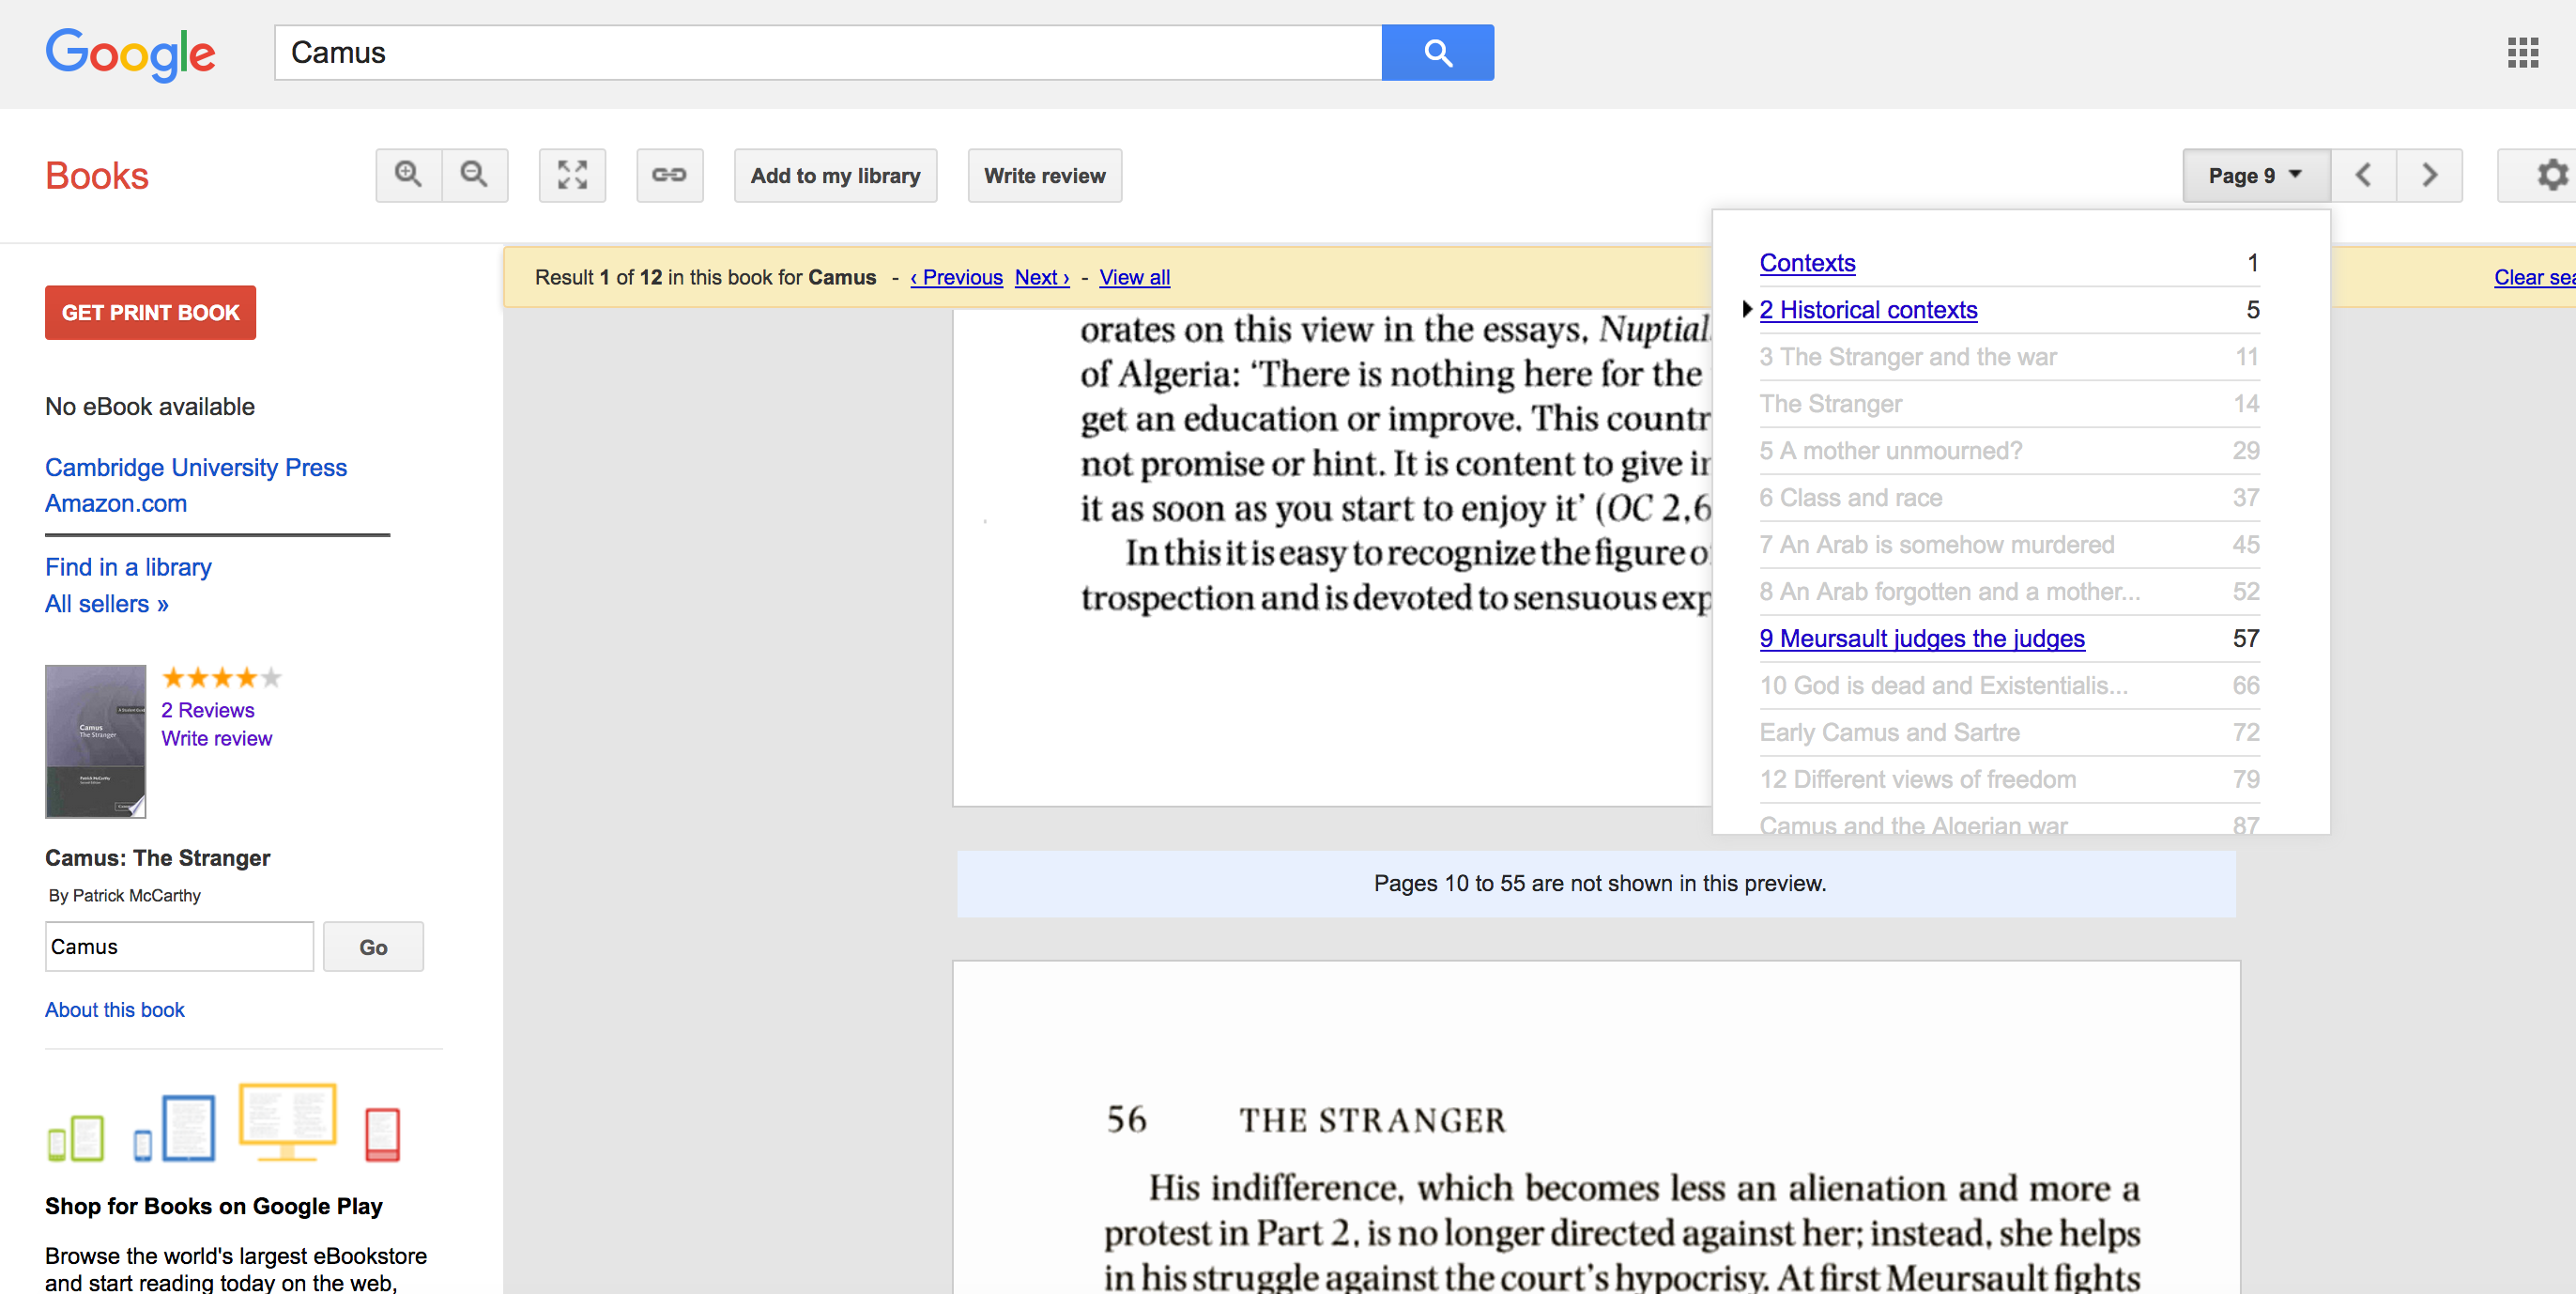
\includegraphics[width=15cm]{googleb}
\caption{Affichage d'un résultat \textit{Google Books}, capture d'écran}
\end{figure}

Passés les débuts rapides et presque \inquote{agressifs} de l'initiative, le droit d'auteur est néanmoins avancé pour justifier le récent ralentissement de l'entreprise et une nouvelle prédilection pour la numérisation d'ouvrages libres de droit\footcite{thylstrup_politics_2018}\footcite{weiss_examining_2016}\footcite{noauthor_viewpoint_nodate}. 

Les débuts sont caractérisés par de nombreux problèmes relatifs à la qualité des métadonnées et des images\footcite{hoffmann_google_2016}. Les langues non romanes sont sous-représentées et les spécificités propres à d'autres histoires littéraires (telles que celles japonaises où les livres sont construits sur d'autres logiques que celles européennes) sont difficilement prises en compte dans les processus de numérisation\footcite{weiss_examining_2016}. Les biais dans la construction des collections sont hérités des bibliothèques partenaires\footcite{weiss_assessing_2013}. De nombreux problèmes sont également constatés concernant la gestion des ouvrages en plusieurs volumes. En vérité, par rapport aux standards élevés des bibliothèques, \textit{Google Books} a du mal à faire concurrence. Cela ne signifie pas qu'il réussit moins bien son objectif de desservir le plus grand nombre, puisqu'il permet d'accéder aux recherches au sein de l'environnement Google.

Google ne partage pas publiquement les processus et les algorithmes de traitement de ces données\footcite{hoffmann_google_2016}. La firme se charge du transport des documents vers le lieu de numérisation, puis restitue les données enrichies une fois numérisées, en garantissant leur intégrité. Certaines bibliothèques témoignent d'un rythme de numérisation de quelques 5000 livres par mois\footcite{association_pour_le_patrimoine_naturel_et_culturel_du_canton_de_vaud_patrimoine_2012}.

La préservation sur le long-terme n'étant pas sa priorité, la firme remet tout de même une copie des fichiers aux institutions afin qu'elles puissent y veiller\footcite{leetaru_mass_2008}, pour autant que ces fichiers demeurent stockés sur les serveurs de l'institution\footcite{association_pour_le_patrimoine_naturel_et_culturel_du_canton_de_vaud_patrimoine_2012}. 

Contrairement aux initiatives publiques, Google n'a pas le souci d'inclure l'usager dans le déploiement de \textit{Google Books}. Il a démontré qu'il était capable de réagir et d'intégrer certaines critiques (notamment celles levées dans les premières années du projet qui reprochaient la mauvaise qualité de la numérisation), mais n'est pas prêt à ouvrir son projet plus largement aux besoins des individus\footcite{jones_public_2017}, qui sont limités au rôle de critiques. Les développements technologiques semblent être prioritaires\footcite{hoffmann_google_2016}. 

Sa quête de profit le pousse également à limiter les usages commerciaux faits par la suite et prévient le référencement des titres numérisés par d'autres moteurs de recherche\footcite{clavert_histoire_2013}\footcite{moatti_bibliotheque_2012}. La firme semble cependant largement autoriser les usages pour la recherche\footcite{leetaru_mass_2008}. 

L'initiative de \textit{Google Books} ne laisse personne indifférent, organisant dès le départ le monde en deux camps, celui des partenaires et celui des opposants. Google est entre-temps devenu un géant de l'information, dont le monopole et le non-respect de la protection des données des utilisateurs suscitent autant la crainte que l'admiration\footcite{clavert_histoire_2013}. De ce clivage va naître la plupart des projets de numérisation de masse du 21\up{e} siècle\footcite{thylstrup_politics_2018}. 

En 2018, quelques \textbf{30 millions} de livres ont été numérisés par cette initiative\footcite{thylstrup_politics_2018} et le fonds continue de croître. 

\newpage

\begin{table}[H]
\centering
\begin{tabular}{|l|l|}
\hline
\rowcolor[HTML]{2E1A46} 
{\color[HTML]{FFFFFF} \textbf{Enjeux}}                                                                                   & {\color[HTML]{FFFFFF} \textbf{Réponses de Google}}                                                                                                                                                                                                                                                                                                                                                                                                                                                                                                                                                         \\ \hline
{\color[HTML]{2E1A46} \textbf{\begin{tabular}[c]{@{}l@{}}Amener différents\\ acteurs à collaborer\end{tabular}}}         & \begin{tabular}[c]{@{}l@{}}Chaque contrat est négocié au cas \\ par cas, mais Google impose certaines règles.\\ Un contrat avec Google n'empêche pas la \\ poursuite d'autres projets de numérisation mais \\ prévient certains usages commerciaux.\end{tabular}                                                                                                                                                                                                                                                                              \\ \hline
{\color[HTML]{2E1A46} \textbf{\begin{tabular}[c]{@{}l@{}}Financement et \\ partenariats \\ public-privé\end{tabular}}} & \begin{tabular}[c]{@{}l@{}}Les profits générés par Google suffisent à couvrir les\\ frais des projets de numérisation. Nul besoin de \\ trouver d'autres partenariats financiers.\end{tabular}                                                                                                                                                                                                                                                                                                                                                                                                            \\ \hline
{\color[HTML]{2E1A46} \textbf{Droit d'auteur}}                                                                           & \begin{tabular}[c]{@{}l@{}}Google a gagné plusieurs procès contre la guilde \\ des auteurs aux États-Unis. Toutefois, ces attaques\\ incessantes sont souvent évoquées comme raison \\ aux choix de numériser des ouvrages libres de droit, \\ caractérisant les plus récentes initiatives.\end{tabular}                                                                                                                                                                                                                                                                                                  \\ \hline
{\color[HTML]{2E1A46} \textbf{\begin{tabular}[c]{@{}l@{}}Sortir des silos : \\ enjeux techniques\end{tabular}}}          & \begin{tabular}[c]{@{}l@{}}Déploiement de centres de numérisation et dépôt \\ de divers brevets visant à accélérer les processus \\ (scanners, mélodie aidant à la concentration, \\ automatisation etc.).\\ Si Google est plutôt transparent sur les contrats de \\ numérisation, il protège farouchement les \\ technologies associées, les centres de numérisation \\ ne sont pas visitables. Comme le projet est inclus dans\\ l'environnement de recherche le plus utilisé, les \\ ouvrages numérisés bénéficient d'une grande\\ visibilité et sont accessibles dans plusieurs langues.\end{tabular} \\ \hline
{\color[HTML]{2E1A46} \textbf{\begin{tabular}[c]{@{}l@{}}Sortir des silos : \\ enjeux sur le \\ contenu\end{tabular}}}   & \begin{tabular}[c]{@{}l@{}}Alors même que le projet a pour objectif de tout\\ numériser, sans sélection préalable, certains choix\\ ont été faits, qui le sortent de cette neutralité.\\ En choisissant les plus grands et prestigieux\\ établissements culturels, Google a reproduit \\ leurs biais, privilégiant les ouvrages scientifiques et \\ classiques au détriment de la littérature populaire. \\ Le projet se consacre également à la seule \\ numérisation de livres et privilégie les partenariats \\ avec des institutions dont les ouvrages sont en langue\\ romane.\end{tabular}          \\ \hline
{\color[HTML]{2E1A46} \textbf{\begin{tabular}[c]{@{}l@{}}Stockage sur le \\ long-terme - \\ préservation\end{tabular}}}  & \begin{tabular}[c]{@{}l@{}}La démarche de Google est une mise à disposition. La\\ qualité des données est trop variable pour prétendre\\ travailler à leur préservation, cette\\ responsabilité est laissée aux institutions partenaires.\end{tabular}                                                                                                                                                                                                                                                                                                                                                    \\ \hline
\end{tabular}
\caption {Les réponses de \textit{Google Books} aux enjeux de la numérisation}
\end{table}
%====== HathiTrust
\subsection{HathiTrust}

Initié en 2006 sous l'impulsion de l'université du Michigan, qui propose aux autres bibliothèques partenaires de \textit{Google Books}\footnote{Comme nous l'avons mentionné plus haut, Google s'inscrit dans une logique d'accès et ne se focalise pas sur le stockage sur le long-terme.} de développer un dépôt commun pour le stockage sur le long-terme des ouvrages numérisés\footcite{noauthor_viewpoint_nodate}. Les missions d'\textit{HathiTrust} sont de contribuer à la recherche, l'éducation et le bien commun en rassemblant, organisant, préservant et rendant accessible, de manière collective et collaborative, les données de la connaissance humaine\footcite{hathitrust_digital_library_charting_nodate}. Ainsi, au-delà de l'objectif de préservation, l'initiative se soucie de leur accessibilité dans le respect du cadre légal, afin de répondre aux besoins de la communauté scientifique : \inquote{\textit{It represents an example of a \inquote{light archive}, meaning, that the repository also functions as a digital library and provides access to some of their collections.}}\footcite[p.275]{xie_discover_2016} Le nom de la plateforme fait écho aux ambitions de ce projet, puisque \textit{Hathi} signifie éléphant en indien, animal connu pour sa mémoire, force et sagesse\footcite{xie_discover_2016}.

\begin{figure}[H]% force à placer l'image au sein de notre balise figure
\centering
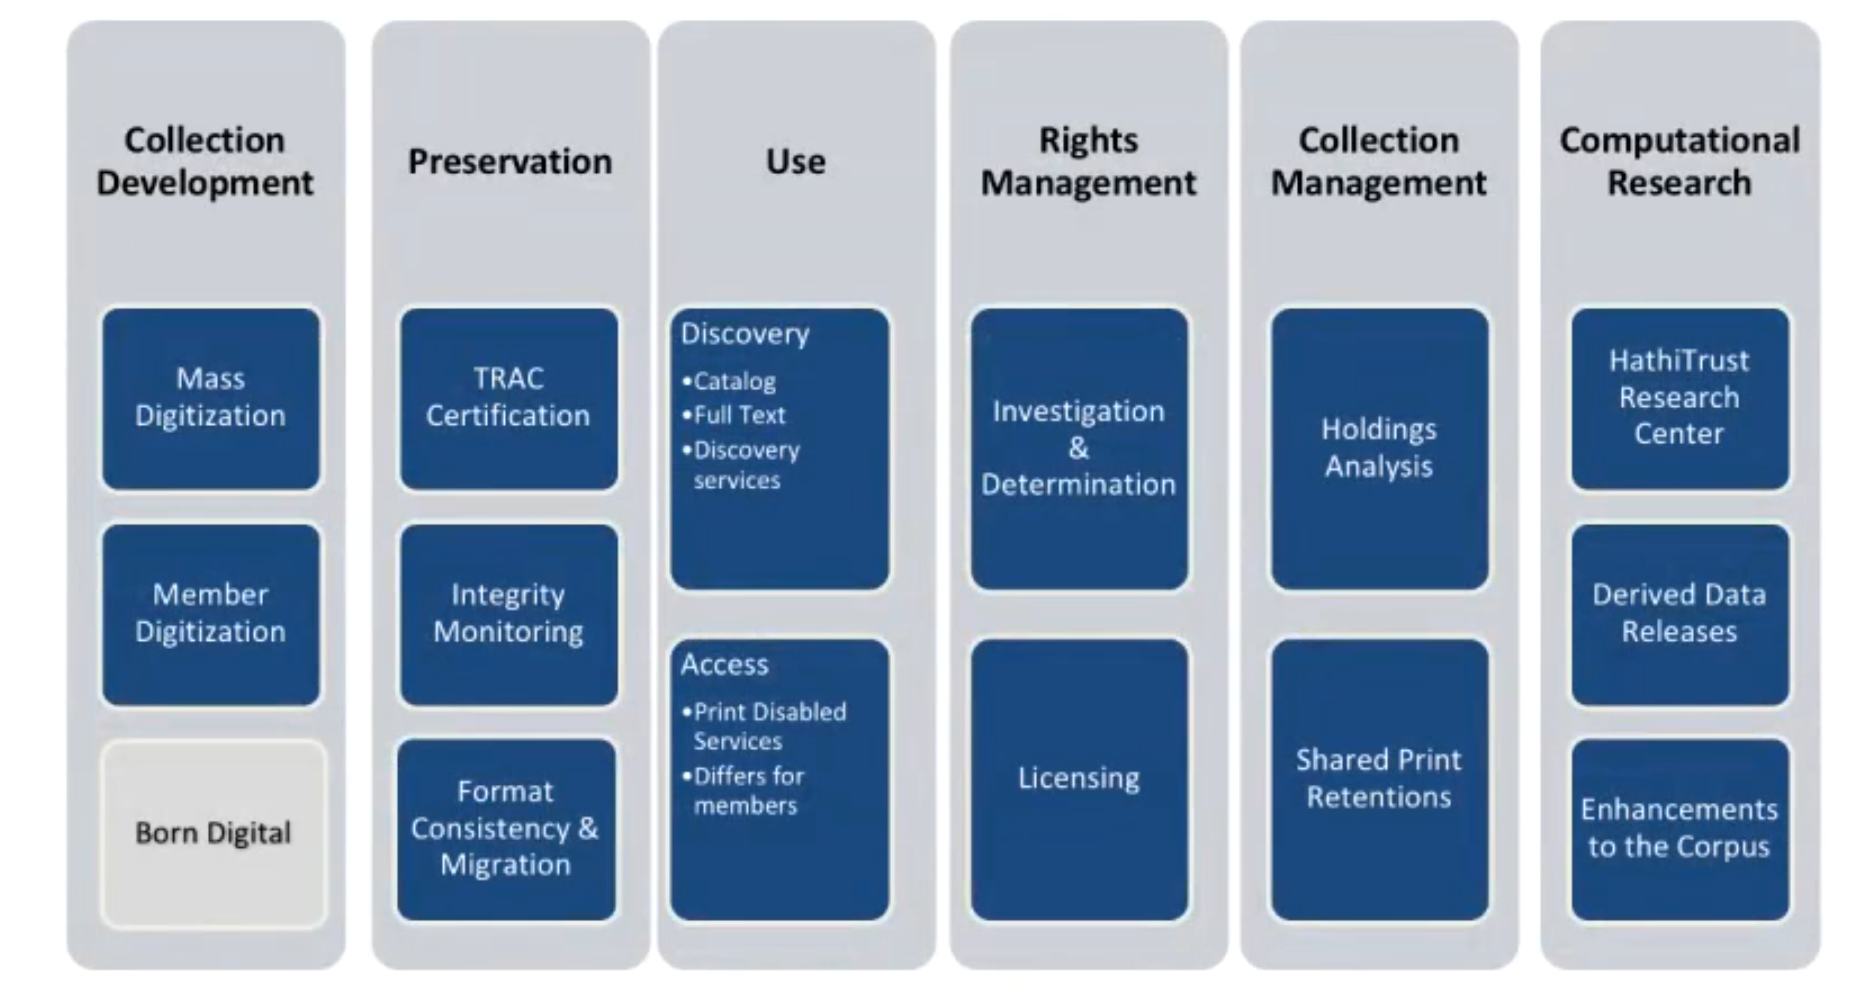
\includegraphics[width=15cm]{hathigoals}
\caption{Résumé des différentes activités entreprises par \textit{HathiTrust}, capture d'écran}
\end{figure}

La plateforme, inaugurée en 2008, propose des livres, articles de journaux sous licences ou libres de droit. Voulue indépendante du projet de Google, elle intègre également de nombreuses autres collections découlant de divers projets de numérisation de masse, publics (\textit{Internet Archive}) ou privés (\textit{Microsoft}). \textit{HathiTrust} regroupe plus d'une centaine de bibliothèques partenaires (140) à travers le monde\footcite{obrien_large-scale_2015} et offre un accès à quelques \textbf{seize millions} de documents\footcite{xie_discover_2016}\footcite{hathitrust_digital_library_charting_nodate}. Active dans différents domaines, l'organisation contribue notamment à la poursuite des projets de numérisation au sein des institutions partenaires en permettant le partage des coûts, et à accroître l'accessibilité et l'usage pour la recherche des données préservées. À travers le développement de différents outils et la mise en place du centre pour les recherches analytiques de \textit{the HathiTrust Research Center Analytics}, l'initiative soutient les travaux de recherches d'envergure conduits dans un objectif scientifique et par des organisations à but non lucratifs\footcite{hathitrust_digital_library_htrc_nodate}.

Pour regrouper les collections des différents partenaires et répondre aux besoins d'interopérabilité, un groupe collaboratif a développé un modèle de gestion des métadonnées visant à regrouper les différentes données des institutions et à en permettre l'exportation dans le format du projet : \textit{Zephir}\footcite{hathitrust_digital_library_zephir_nodate}. Portée par l'expertise des bibliothèques partenaires, la recherche offre des fonctionnalités similaires à celles que l'on peut trouver via les interfaces de ces institutions, permettant de rechercher dans les index (titre, auteur etc.), en plus de la recherche avancée et d'une recherche plein-texte. De la qualité de ses métadonnées, découle la robustesse et les performances de son moteur de recherche\footcite{weiss_using_2014}. L'affichage des résultats est toutefois limité en fonction du droit d'auteur\footcite{lau-suchet_hathitrust_2014}, puisque \textit{HathiTrust} vise avant tout à préserver les collections et s'inscrit moins dans une démarche d'accessibilité universelle. Certains ouvrages soumis au droit d'auteur ne peuvent être recherchés ou certaines fonctionnalités de la plateforme sont réservées aux membres des institutions partenaires (comme le téléchargement pdf des textes libres de droit), ce qui a valu au projet quelques critiques\footcite{wu_building_2011}\footcite{obrien_large-scale_2015}\footcite{xie_discover_2016}. 

L'anglais représente la langue majoritaire dans les collections\footcite{weiss_using_2014}, même si l'initiative poursuit l'objectif de permettre la recherche dans tous les systèmes d'écriture existants (actuellement celle-ci est disponible en caractères cyrilliques, hébreux, grecs, chinois, japonais et coréens)\footcite{lau-suchet_hathitrust_2014}.
\newpage
\begin{figure}[H]% force à placer l'image au sein de notre balise figure
\centering
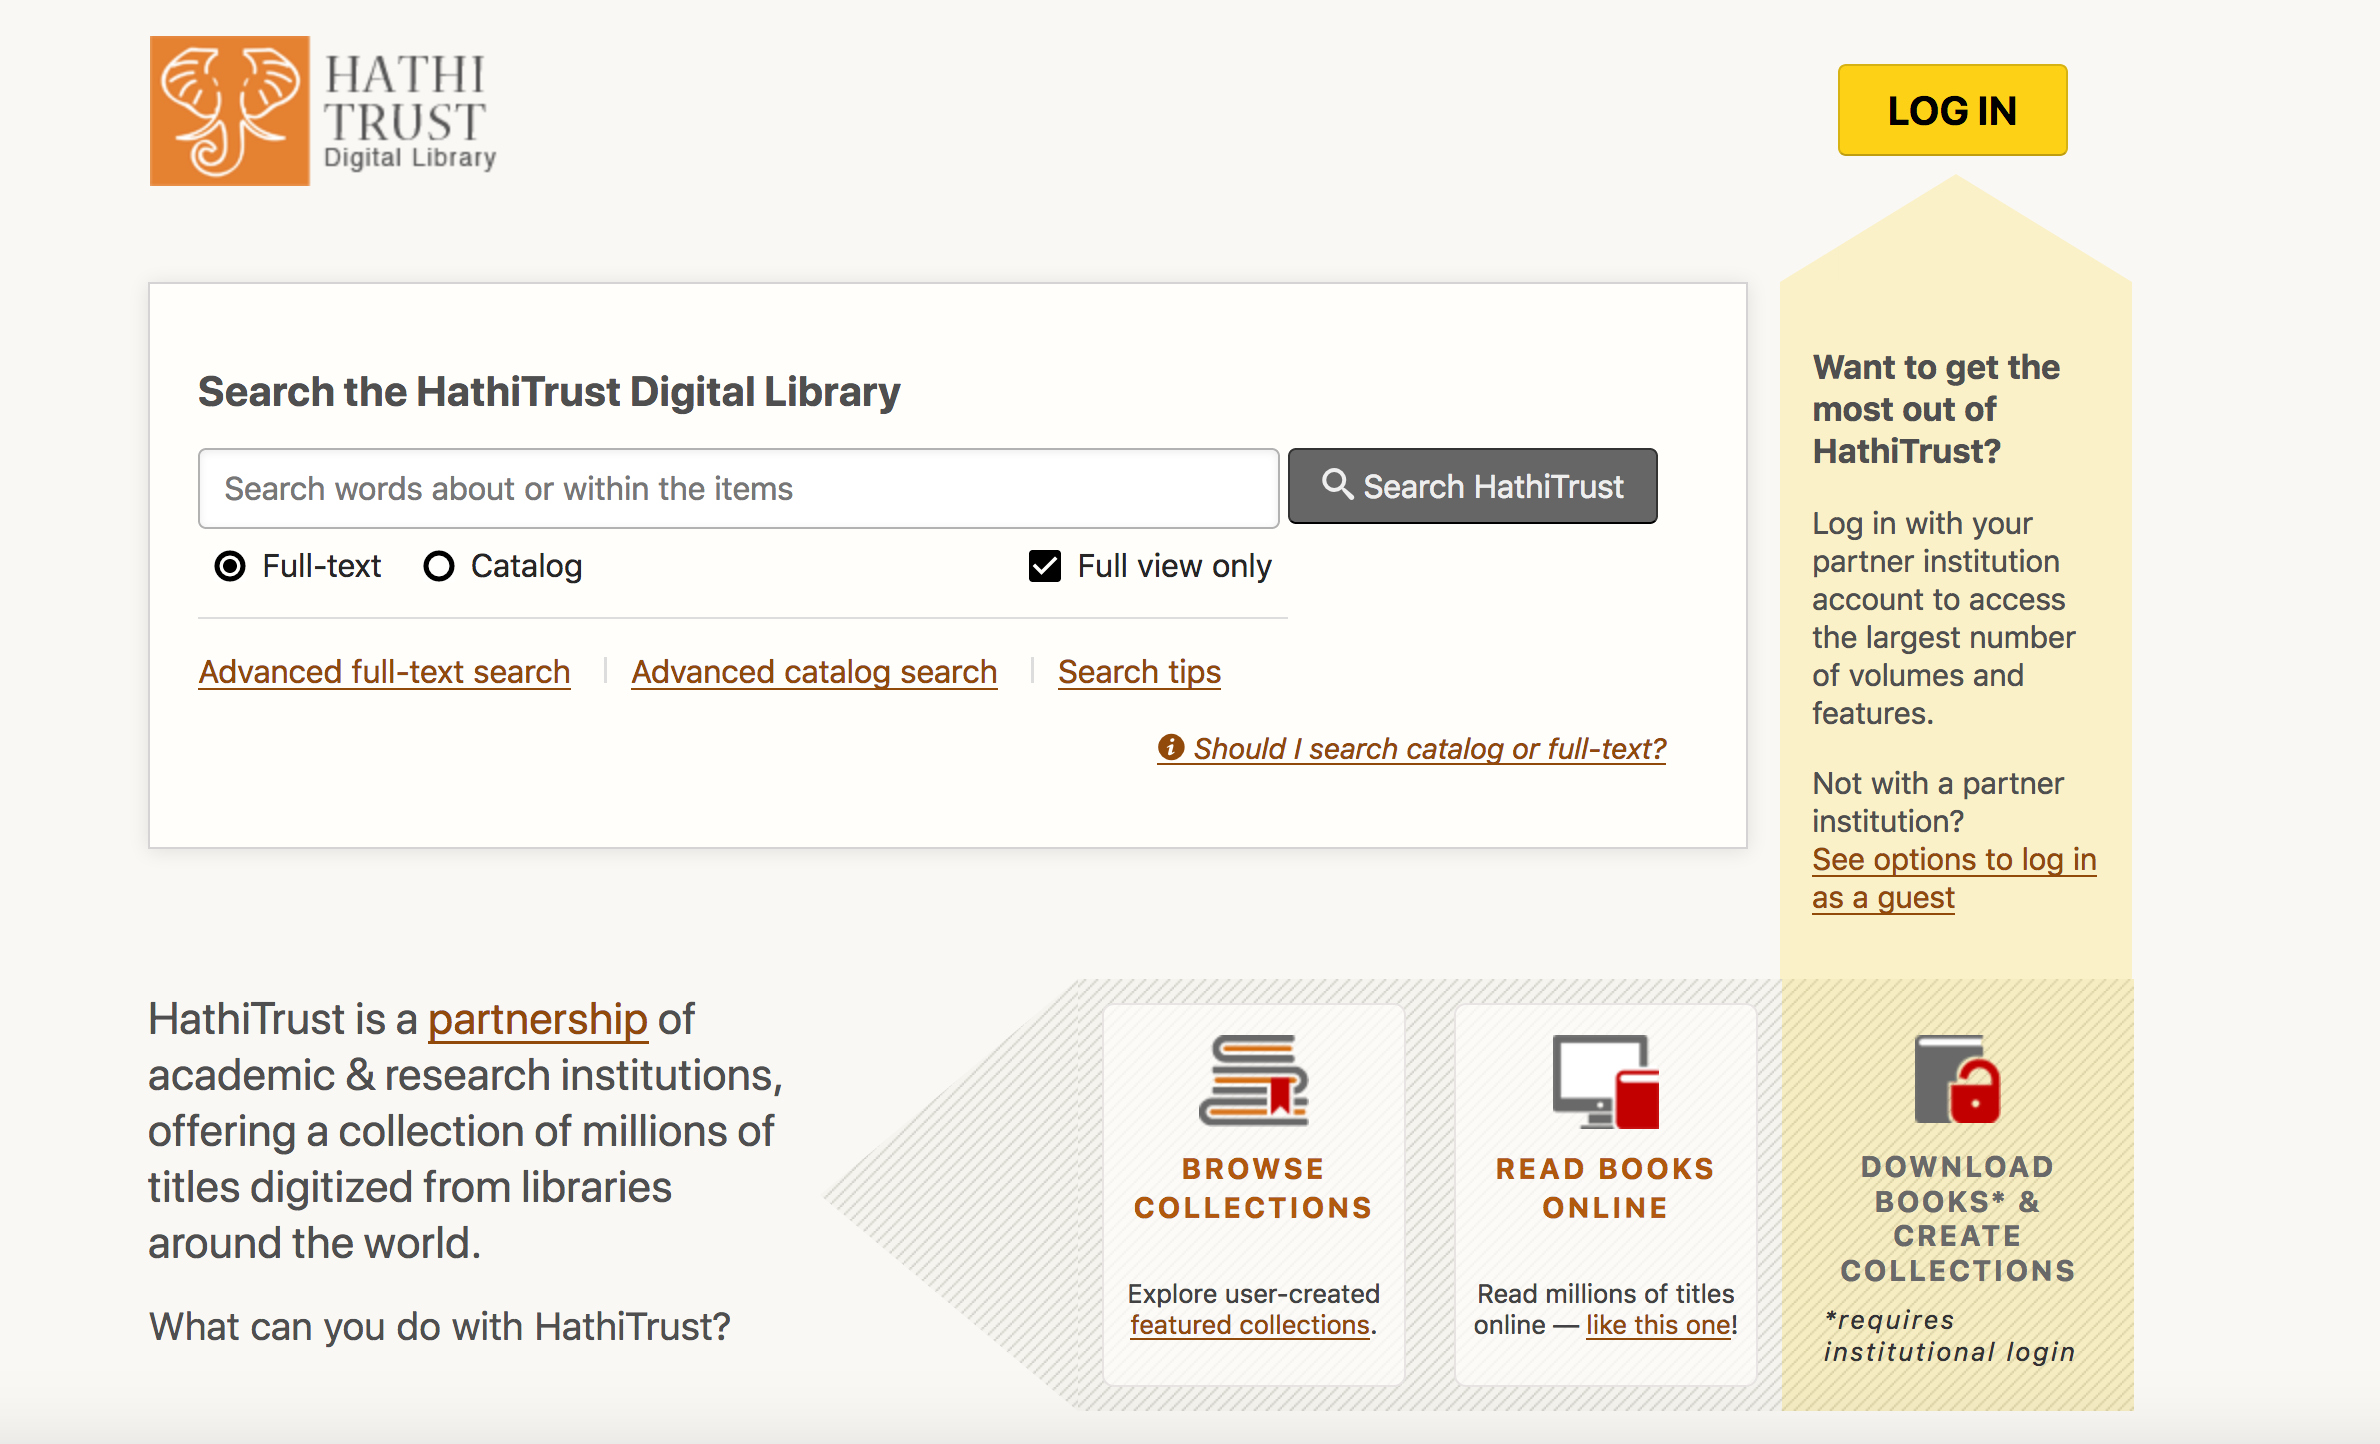
\includegraphics[width=15cm]{hathiface}
\caption{Page d'accueil de la plateforme d'\textit{HathiTrust}, capture d'écran}
\end{figure}

À l'inverse de Google, \textit{HathiTrust} sait gérer les ouvrages en plusieurs volumes, ce qui contribue à leurs découvertes\footcite{weiss_examining_2016} et s'attèle à vérifier le statut d'un document lorsque des doutes liés au droit d'auteur persistent\footcite{weiss_examining_2016}. La collaboration entre institutions partenaires est réalisée dans la plus grande transparence, et le site internet, mis à jour régulièrement, offre les derniers détails sur les décisions stratégiques soumises à l'approbation générale (dont les directions stratégiques envisagées pour la période 2019-2023)\footcite{hathitrust_digital_library_charting_nodate}. \textit{HathiTrust} développe des interfaces spécialement destinées aux personnes en situation de handicap\footcite{hathitrust_digital_library_charting_nodate}, ce qui contribue à accroître l'accessibilité de ses collections.
\newpage
\begin{table}[H]
\centering
\begin{tabular}{|l|l|}
\hline
\rowcolor[HTML]{2E1A46} 
{\color[HTML]{FFFFFF} \textbf{Enjeux}}                                                                                   & {\color[HTML]{FFFFFF} \textbf{Réponses de HathiTrust}}                                                                                                                                                                                                                                                                                                                                                                                                                                                                                                                                         \\ \hline
{\color[HTML]{2E1A46} \textbf{\begin{tabular}[c]{@{}l@{}}Amener différents\\ acteurs à collaborer\end{tabular}}}         & \begin{tabular}[c]{@{}l@{}}Projet collaboratif, porté par quelques 140 \\ bibliothèques partenaires. Une complète transparence\\ semble être garante d'une cohésion d'ensemble.\end{tabular}                                                                                                                                                                                                                                                                                                                                                                                                   \\ \hline
{\color[HTML]{2E1A46} \textbf{\begin{tabular}[c]{@{}l@{}}Financement et \\ partenariats \\ public-privé\end{tabular}}} & \begin{tabular}[c]{@{}l@{}}Les bibliothèques financent les infrastructures, selon une \\ somme calculée sur différents facteurs à la fois liés aux \\ collections de l'institution mais également à la taille du \\ réseau et au pourcentage d'\oe{}uvres sous droits. Le projet \\ ne semble pas recourir à des financements privés, mais\\ bénéficie de leurs entreprises de numérisation.\end{tabular}                                                                                                                                                                                          \\ \hline
{\color[HTML]{2E1A46} \textbf{Droit d'auteur}}                                                                           & \begin{tabular}[c]{@{}l@{}}HathiTrust a gagné son procès contre la guilde \\ des auteurs aux États-Unis. Il limite l'accès plein-texte des\\ ouvrages sous droits et entreprend de véritables recherches\\ afin de déterminer si des licences s'appliquent.\end{tabular}                                                                                                                                                                                                                                                                                                                       \\ \hline
{\color[HTML]{2E1A46} \textbf{\begin{tabular}[c]{@{}l@{}}Sortir des silos : \\ enjeux techniques\end{tabular}}}          & \begin{tabular}[c]{@{}l@{}}La qualité des métadonnées caractérisent le projet, favorisant\\ l'efficacité du moteur de recherche. Un système de gestion\\ dédié a été développé : \textit{Zephir}. Ce dernier attribue un score\\ à chaque fichier de métadonnées en fonction des informations\\ trouvées dans les différents champs de métadonnées. Si ce \\ score est trop bas, l'institution sera priée de corriger les \\ éléments manquants ou une notice développée par un autre\\ partenaire sera utilisée. Différentes APIs favorisent l'accès \\ aux métadonnées ou aux documents.\end{tabular} \\ \hline
{\color[HTML]{2E1A46} \textbf{\begin{tabular}[c]{@{}l@{}}Sortir des silos : \\ enjeux sur le \\ contenu\end{tabular}}}   & \begin{tabular}[c]{@{}l@{}}Le projet est motivé par des besoins académiques et ses\\ collections portent de fait le même biais scientifique que\\ les institutions partenaires. On observe une plus\\ forte représentation des ouvrages en langue anglaise. \\ Très peu d'institutions sont partenaires en dehors de\\ ce milieu linguistique. Les formats des collections sont \\ limités aux livres et articles de presse. Le projet rassemblant \\ des données préalablement numérisées, ses collections \\ offrent une forte redondance avec celles d'autres initiatives.\end{tabular}     \\ \hline
{\color[HTML]{2E1A46} \textbf{\begin{tabular}[c]{@{}l@{}}Stockage sur le \\ long-terme - \\ préservation\end{tabular}}}  & \begin{tabular}[c]{@{}l@{}}Le point fort du projet. L'infrastructure a été conçue pour \\ garantir la longévité des données et suit les normes récentes. \\ Les métadonnées de provenance et de contexte, et l'intégrité\\ et l'authenticité des documents sont préservés.\end{tabular}                                                                                                                                                                                                                                                                                                        \\ \hline
\end{tabular}
\caption{Les réponses de \textit{HathiTrust} aux enjeux de la numérisation}
\end{table}

\section{Agréger pour mieux valoriser}

%==== Europeana

\subsection{Europeana}

Issue de diverses réactions politiques à l'arrivée de \textit{Google Books}\footnote{En 2004, le Président français Jacques Chirac demande au directeur de la BNF Jean-Noël Jeanneney de lancer un projet européen similaire. Le directeur étant effrayé à la perspective de laisser les lois anglo-saxonnes s'imposer en Europe, il appelle à un effort national de numérisation et à la création d'une infrastructure européenne à même de préserver les différences culturelles des nations. Toutefois Europeana ne s'est pas construit comme une réponse à \inquote{l'invasion américaine}, d'autres voix plus pragmatiques, à l'instar de celle du président de la Commission européenne, José Manuel Barroso, ont argumenté du besoin de créer une économie de la connaissance \cite{thylstrup_politics_2018}}, Europeana est lancée par l'\gls{ue} en 2008, motivée par la perspective de créer une nouvelle économie de la connaissance. Le projet vise à favoriser le partage de contenus de qualités vers une audience européenne, à agrandir le nombre des partenaires afin de toucher toutes les parties concernées et à susciter l'intérêt du public quel qu'il soit, pour les contenus des institutions culturelles et patrimoniales\footcite{europeana_europeana_nodate-2}. La plateforme donne accès à quelques \textbf{58 millions} d'objets numérisés et élargit le spectre de leurs typologies. Les collections multilingues se composent d'images (33.5 millions), de textes (22.8 millions), de fichiers audio (700'000) ou vidéo (1.2 millions) et d'objets 3D (28'000) issus de plus de 3500 institutions\footcite{europeana_europeana_nodate-2}\footcite{xie_discover_2016}\footcite{noauthor_european_2019}.

En temps qu'\gls{agr}, Europeana bénéficie des entreprises de numérisations menées à l'échelle d'une nation ou d'une région, faisant converger les attentes de chacun au sein d'une infrastructure commune : \inquote{\textit{Europeana produces a new form of cultural memory politics that converge national and supranational imaginaries with global information infrastructures}\footcite[p.57]{thylstrup_politics_2018}}.
\newpage
\begin{figure}[H]% force à placer l'image au sein de notre balise figure
\centering
\includegraphics[scale=0.3]{europeana}
\caption{Page d'accueil de l'interface découverte d'Europeana, capture d'écran}
\end{figure}

Bien que se réclamant d'une souveraineté nationale, Europeana travaille avec les grands réseaux du web (Google, Microsoft etc.) pour financer la numérisation des données qui seront rassemblées sur sa plateforme. Présenté comme une initiative européenne, le projet réagit à des règles de privatisation induites par ces partenariats\footcite{thelle_persuasive_2011}. Les frontières entre public-privé tendant à se moduler à travers l'infrastructure, et celles entre institutions et environnement suivent la même logique\footcite[p.63]{thylstrup_politics_2018}. Ce paradoxe sera d'ailleurs souvent critiqué\footcite{thelle_persuasive_2011}\footcite{thelle_persuasive_2011}.

\begin{quotation}
[\textit{Traduction}]
Si Europeana est un projet de numérisation de masse construit autour d'anciennes logiques souveraines, dont le discours officiel valorise l'État nation, en même temps qu'il abolit les frontières en déployant des infrastructures interopérables, la question demeure : quel est le résultat de cet assemblage d'un point de vue culturel ?\footnote{\inquote{\textit{If Europeana is a late-sovereign mass digitization project that maintains discursive ties to the national imaginary at the same time that it undercuts this imaginary by means of networked infrastructure through increased interoperability, the final question is: what does this late-sovereign assemblage produce in cultural terms?}}\cite[p.73]{thylstrup_politics_2018}}
\end{quotation}

Europeana étant un projet sous financement européen, il respecte le droit d'auteur \footnote{par opposition à Google avec son application du \textit{fair use}}, alors même que ce système est très complexe à déployer. Comme l'Europe ne possède pas de législation commune, il navigue entre les différentes particularités nationales, l'émergence d'un marché global et la mouvance du \gls{oa}\footcite{thylstrup_politics_2018}\footcite{weiss_using_2014}. Europeana favorise les contenus en accès libres sous licence \textit{\gls{cc}} CC0\footnote{Licence la moins restrictive, n'obligeant pas à citer la provenance du contenu.}, ce qui pose des problèmes d'application pour certains États (dont la France), plus restrictifs\footcite{noauthor_european_2019}. On retrouve également différentes formes d'affichage en fonction de ces restrictions (accès aux contenus interactifs et aux métadonnées, accès aux contenus statiques et métadonnées, extraits et métadonnées, métadonnées seulement)\footcite{willems_europeana_2015}. Les \oe{}uvres à partir du 20\up{e} siècle sont sous-représentées au profit des \oe{}uvres libres de droit\footcite{dufrene_numerisation_2013}\footcite{stobo_i_2018}.

Pour tenter de répondre à ces différentes contraintes tout en effectuant sa mission, Europeana investit le principe d'interopérabilité : proposant notamment un cadre de publication à destination des institutions directement ou des \gls{agr}s nationaux et thématiques de collections numérisées\footnote{Afin de mieux interagir avec les plateformes et institutions existantes, Europeana a créé en 2012 le \textit{Europeana Aggregator forum}. Ce lieu permet la mise en place d'échanges professionnels et assure l'implication de ces instances stratégiques au sein du projet. Les agrégateurs offrent à leurs institutions partenaires conseils et support dans leurs projets de numérisation concernant le choix les licences ; formats ;  traitement du multilinguisme etc... \cite{europeana_breathing_nodate}. Plus de 2/3 des États membres ont des agrégateurs nationaux \cite{noauthor_european_2019}.} ; une stratégie de contenu ; un modèle de métadonnées suivant les recommandations du web sémantique\footcite{europeana_linked_nodate-1} et proposant un enrichissement à l'aide de vocabulaires contrôlés\footnote{Lexique servant à organiser les connaissances pour favoriser la recherche d'information} ;  des modèles de licences basés sur les \textit{\gls{cc}}. Plusieurs \gls{api}s (dont celles développées par \gls{iiif}) contribuent à l'accessibilité des collections et la naissance de nouveaux produits\footcite{roued-cunliffe_participatory_2017}\footnote{à l'instar de l'\textit{EuropeanaBot}, garant d'une certaine forme de sérendipité, puisque publiant aléatoirement des images issues des collections. \cite{noauthor_europeana_nodate}.}. Les données sont également rendues accessibles via le protocole \gls{oai}\footcite{europeana_everything_nodate}. Soucieuse de garantir une meilleure utilisation des données, Europeana conjointement avec \gls{dpla} et d'autres institutions, fait partie du \textit{RightsStatements.org} Consortium proposant des \inquote{déclarations de droits standardisées pour le patrimoine culturel disponible en ligne}\footcite{noauthor_rightsstatements.org_nodate}. Les institutions peuvent choisir entre 12 déclarations (en cours de traductions dans tous les idiomes européens), favorisant l'usage des fichiers par le public\footcite{noauthor_european_2019}. 

De nombreuses communautés sont impliquées dans Europeana. Le projet s'est construit dans la mouvance des \gls{cs}, dès lors ces communautés participent entre autres aux corrections, transcriptions, classification, contextualisation des données numérisées. L'expérience promue par le projet est de ne pas simplement demander aux utilisateurs de cliquer, mais de leur offrir l'opportunité de prendre une part active dans un projet de recherche\footcite{thylstrup_politics_2018}. Ce souci d'impliquer l'utilisateur se retrouve dans le développement de la plateforme et des services, héritage probable des pratiques mises en place au sein des institutions partenaires\footcite{jones_public_2017}. 

Pour améliorer l'expérience utilisateur et lui permettre de trouver son chemin face aux collections foisonnantes, des expositions virtuelles ont été créées\footcite{europeana_europeana_nodate-2}, la recherche peut se faire dans toutes les langues européennes mais les métadonnées, proposées en résultat ne sont pas traduites\footcite{noauthor_european_2019}. Europeana propose deux interfaces différentes, s'adressant d'un côté à l'utilisateur \inquote{grand public} et mettant en avant la découverte, ou interagissant en toute transparence sur sa plateforme professionnelle avec les partenaires du réseau et les entités ou individus motivés à profiter pleinement des opportunités offertes par ses collections massives (éducation, recherche, industries etc.)\footcite{ioana_roiu_cristina_family_nodate}. L'interface professionnelle décrit précisément l'organisation, les spécificités techniques et propose des accompagnements ciblés selon si l'on se positionne en tant que partenaire du réseau, chercheur, ou futur exploitant\footcite{europeana_europeana_nodate-2}. 

Europeana propose depuis les débuts des interfaces mobiles, ce qui est important pour le projet, car la plupart de son trafic provient des portables\footcite{xie_discover_2016}.
 \newpage
\begin{figure}[H]% force à placer l'image au sein de notre balise figure
\centering
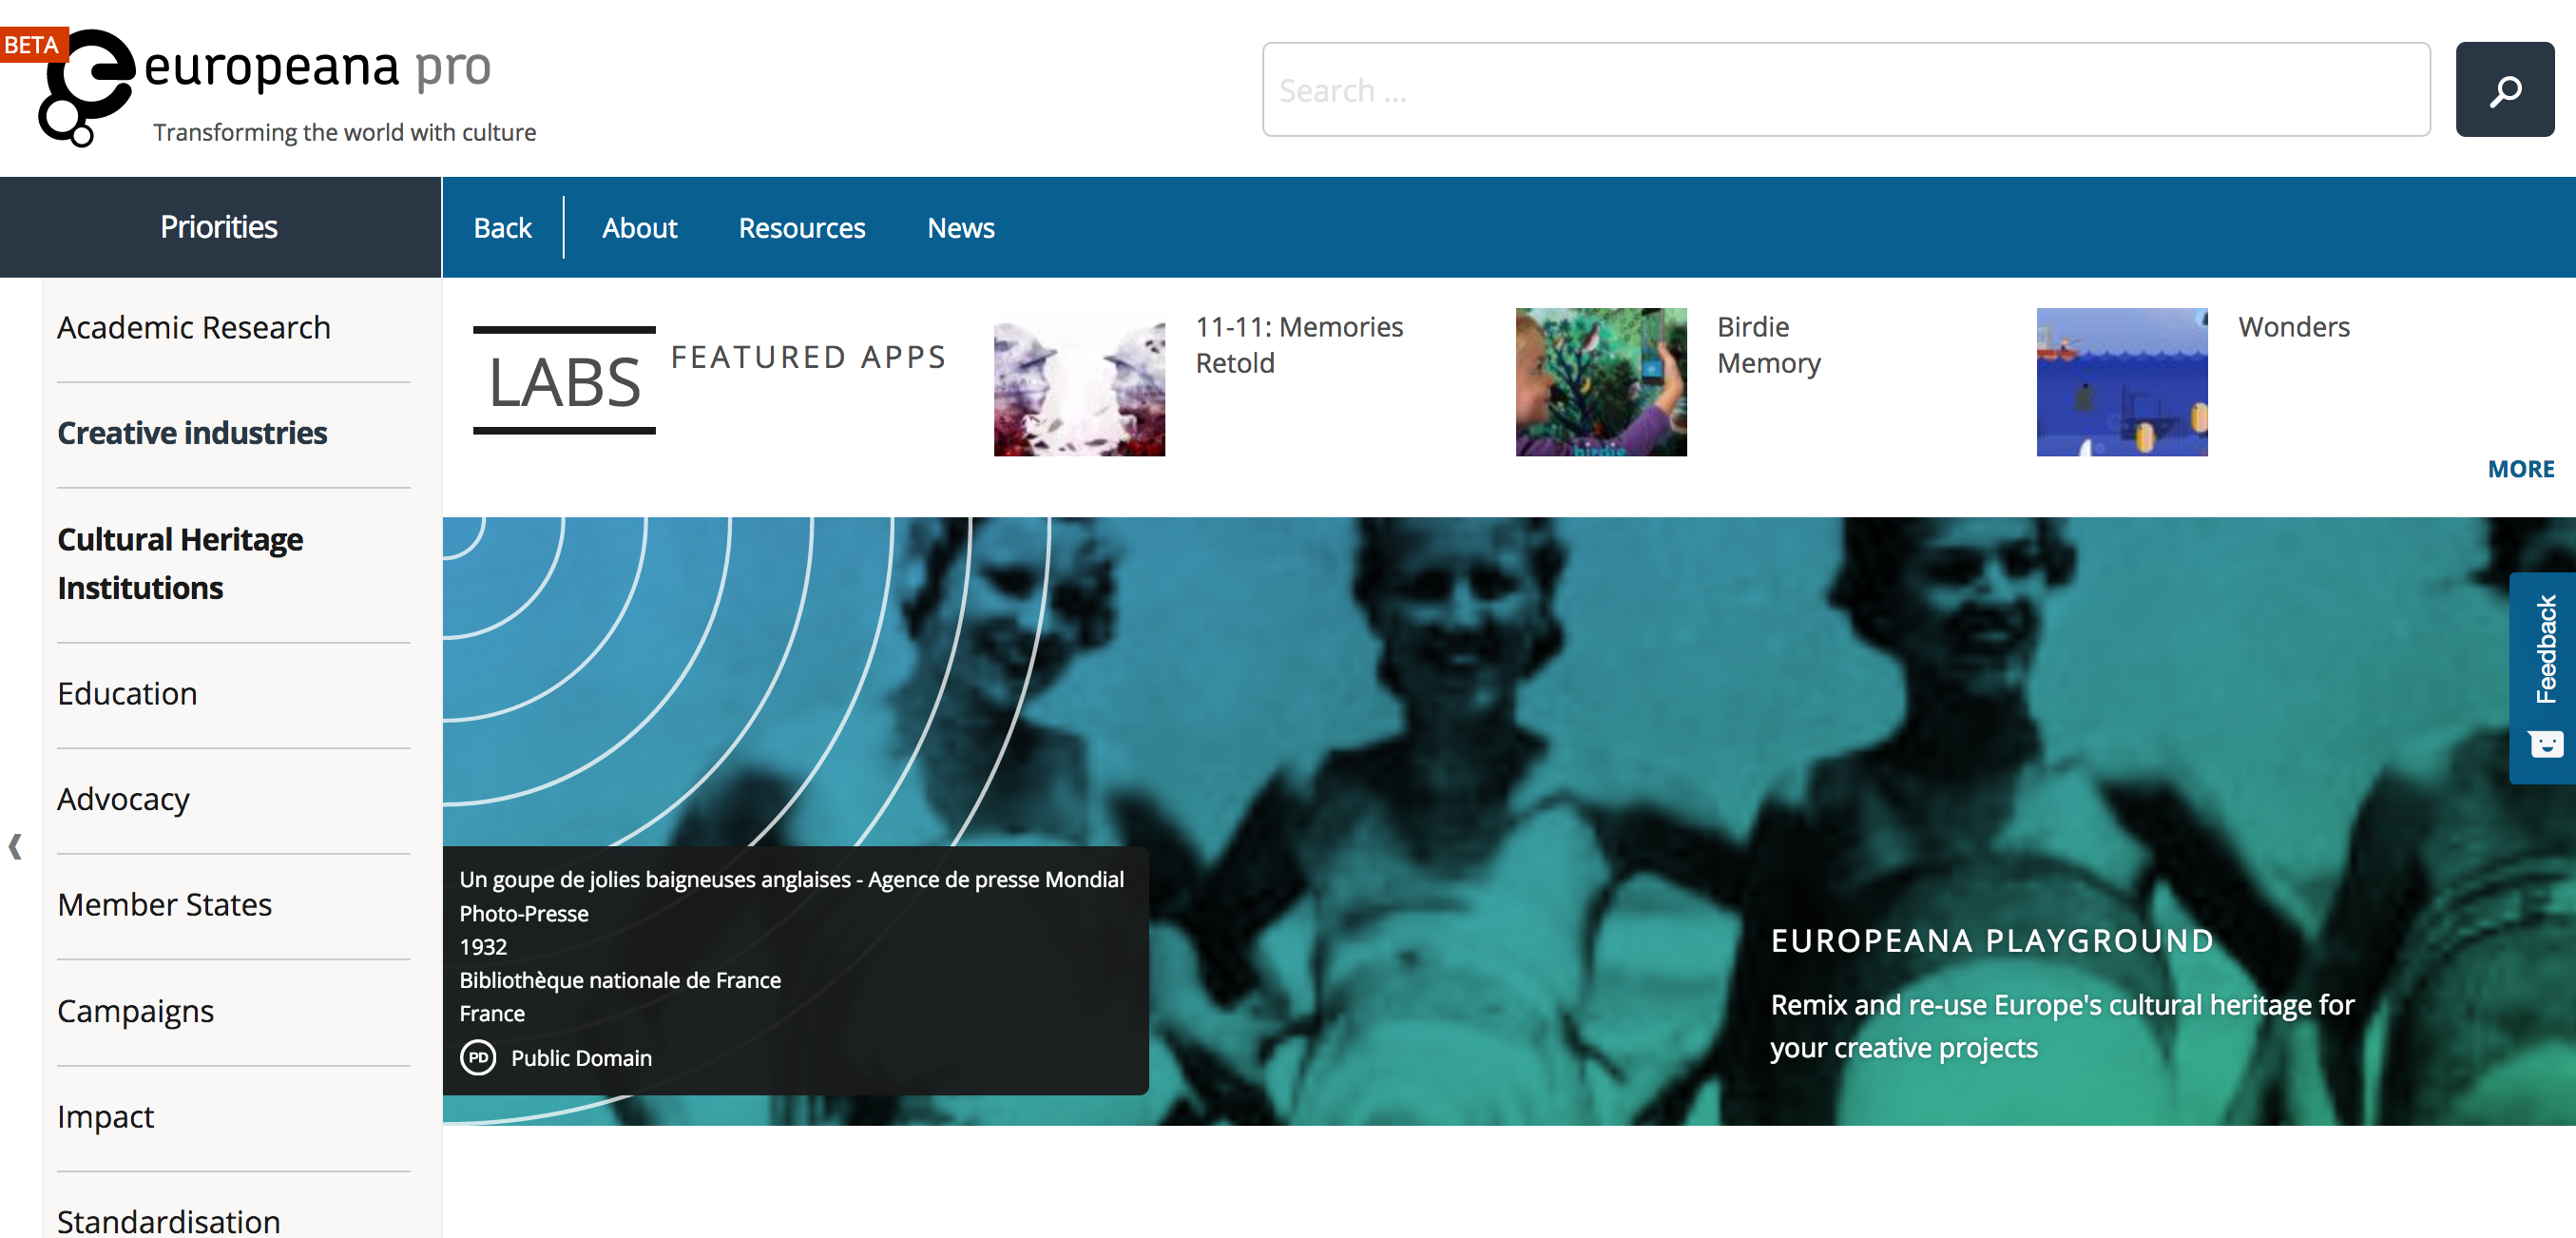
\includegraphics[width=15cm]{europeanapro}
\caption{Page d'accueil de l'interface professionnelle d'Europeana, capture d'écran}
\end{figure}

Se voulant reflet du patrimoine culturel européen, ses collections n'en sont toutefois pas pleinement représentatives. Certains pays ont moins développé la numérisation (biais géographique), certaines typologies d'objets sont sous-représentées, les collections héritent des biais des institutions partenaires\footcite{thylstrup_politics_2018}. Ce qui amènera un responsable d'Europeana à caractériser, en 2010, la différence entre Google et Europeana, par le fait que d'un côté l'usager accède à tout, alors que de l'autre les collections ont été soigneusement sélectionnées par les institutions en vue de leur numérisation\footcite{thelle_persuasive_2011}. Toutefois Europeana tente de proposer de nouvelles formes de numérisation, impliquant le citoyen dans le processus de sélection\footnote{Dans le cadre du projet Europeana 1914-1918, les individus ont été sollicités afin de créer une archive de la Première Guerre Mondiale basée sur leurs images et écrits familiaux \cite{ioana_roiu_cristina_family_nodate}.}, et a mis en place une stratégie de contenu visant à pallier aux manques des collections\footcite{europeana_everything_nodate}.

Europeana n'est pas responsable du stockage sur le long-terme des collections numérisées. Une forte disparité est constatée au niveau européen concernant l'existence de législations relatives à la préservation des données. Cette dernière est souvent dépendante du bon vouloir des institutions\footcite{noauthor_european_2019}.

Malgré son ancrage européen, Europeana est embranchée dans un écosystème Google, laissant le projet à la merci de changements de sa stratégie de référencement et par conséquent face au risque de perdre en visibilité\footcite{thylstrup_politics_2018}. Afin de mieux traiter la richesse des langues européennes, le projet a d'ailleurs intégré une fonction Google, \textit{Google Translate}\footcite{thelle_persuasive_2011}. Depuis 2011, les bibliothèques européennes signataires d'un accord de numérisation avec Google voient leurs documents indexés par Europeana\footcite{moatti_bibliotheque_2012}.

L'\gls{ue} a récemment fixé les nouvelles priorités pour Europeana, qui visent à : développer le multilinguisme de la plateforme ; améliorer la valorisation des collections et proposer de nouveaux services de découverte ; mieux prendre en compte les besoins des petites institutions\footcite{noauthor_european_2019}.

\newpage
\begin{table}[H]
\centering
\begin{tabular}{|l|l|}
\hline
\rowcolor[HTML]{2E1A46} 
{\color[HTML]{FFFFFF} \textbf{Enjeux}}                                                                                   & {\color[HTML]{FFFFFF} \textbf{Réponses d'Europeana}}                                                                                                                                                                                                                                                                                                                                                                                                                                                     \\ \hline
{\color[HTML]{2E1A46} \textbf{\begin{tabular}[c]{@{}l@{}}Amener différents\\ acteurs à collaborer\end{tabular}}}         & \begin{tabular}[c]{@{}l@{}}Une grande transparence et l'élaboration du cadre technique\\ en collaboration étroite avec les partenaires semblent être\\ garants d'une bonne collaboration. De nombreux groupes\\ de travail impliquant les institutions contribuent aux \\ évolutions du projet. Les agrégateurs nationaux ou thématiques\\ sont intégrés au sein d'un forum, favorisant les échanges. Le \\ grand public devient partenaire des projets de recherche.\end{tabular}                      \\ \hline
{\color[HTML]{2E1A46} \textbf{\begin{tabular}[c]{@{}l@{}}Financement et \\ partenariats \\ public-privé\end{tabular}}} & \begin{tabular}[c]{@{}l@{}}Comme la plupart des projets de numérisation sont\\ conduits de manière décentralisées par les institutions,\\ ces dernières se tournent vers des institutions\\ privées (Google, Microsoft etc.) pour les financer. \\ L'Europe finance l'infrastructure et quelques projets de \\ numérisation ciblés.\end{tabular}                                                                                                                                                         \\ \hline
{\color[HTML]{2E1A46} \textbf{Droit d'auteur}}                                                                           & \begin{tabular}[c]{@{}l@{}}Le projet agit dans la légalité et applique des licences\\ et restrictions aux \oe{}uvres sous droit.\\ Un cadre de publication règle les conditions d'échange\\ des métadonnées et s'assure que la mention de la licence \\ y figure. Les licences \textit{Creative Commons} sont privilégiées. \\ Membre du \textit{RightsStatements}, le projet propose des \\ déclarations de droit standardisées. Différentes formes \\ d'affichage garantissent un accès légal aux collections.\end{tabular} \\ \hline
{\color[HTML]{2E1A46} \textbf{\begin{tabular}[c]{@{}l@{}}Sortir des silos : \\ enjeux techniques\end{tabular}}}          & \begin{tabular}[c]{@{}l@{}}Un cadre de publication contenant un modèle de \\ métadonnées a été développé. Différentes APIs (dont IIIF) \\ sont déployées, le protocole OAI-PMH est disponible, les\\ métadonnées sont exposées suivant les principes du web\\ sémantique et enrichies grâce à des vocabulaires contrôlés.\end{tabular}                                                                                                                                                                   \\ \hline
{\color[HTML]{2E1A46} \textbf{\begin{tabular}[c]{@{}l@{}}Sortir des silos : \\ enjeux sur le \\ contenu\end{tabular}}}   & \begin{tabular}[c]{@{}l@{}}Conscient des biais liés aux formats, à la géographie et\\ à l'héritage des institutions partenaires, le projet a mis en \\ place une stratégie de contenu afin de pallier aux manques\\ constatés. De nombreux formats de documents sont disponibles,\\ dont des fichiers audio, vidéo et 3D. Les documents sont\\ multilingues mais le français est sur-représenté.\end{tabular}                                                                                            \\ \hline
{\color[HTML]{2E1A46} \textbf{\begin{tabular}[c]{@{}l@{}}Stockage sur le \\ long-terme - \\ préservation\end{tabular}}}  & \begin{tabular}[c]{@{}l@{}}Europeana n'a pas vocation à stocker directement les données,\\ (cette responsabilité est laissée aux institutions) \\ toutefois les critères de qualité imposés aux métadonnées \\ contribuent à la préservation de l'authenticité et \\ de l'intégrité des documents.\end{tabular}                                                                                                                                                                                              \\ \hline
\end{tabular}
\caption {Les réponses d'Europeana aux enjeux de la numérisation}
\end{table}

 
\subsection{Digital Public Library of America}

La \textit{Digital Public Library of America} ou \gls{dpla}, pensée dès 2010 et officiellement lancée en 2013 vise à rendre le contenu des institutions culturelles et patrimoniales états-uniennes accessible à tous. Deux programmes ont été mis en place pour répondre à cette mission : l'agrégation des données numériques des institutions de tous les États-Unis et un service d'ebooks\footcite{digital_public_library_of_america_strategic_nodate}\footcite{digital_public_library_of_america_history_nodate}. Ce projet est en grande partie dû aux travaux intellectuels du \textit{Berkman Klein Center for Internet and Society\footnote{La mission de ce centre est notamment d'explorer le cyberespace et d'identifier le besoin de nouvelles législations ou des ajustements de celles existantes.}} de l'université d'Harvard et de grands théoriciens du numérique, et des bibliothèques, qui ont travaillé à le positionner comme une alternative publique à l'infrastructure privée de \textit{Google Books}\footcite{thylstrup_politics_2018}. Cependant, comme dans toutes les initiatives de numérisation de masse, la notion de \inquote{public} suscite de nombreuses controverses, puisque l'on reproche à ces projets de détourner l'argent autrement réservé aux infrastructures plus petites\footcite{thylstrup_politics_2018}. 

Le réseau rassemble quelques 41 États, plus de 4000 institutions et permet de découvrir à travers sa plateforme plus de \textbf{30 millions} d'objets de différentes typologies (images, cartes, fichiers audio, manuscrits, \oe{}uvres muséales etc.)\footcite{digital_public_library_of_america_strategic_nodate}. Au même titre qu'Europeana, le projet n'héberge pas ces données, mais offre un portail permettant d'y accéder\footcite{pomerantz_metadata_2015}\footcite{xie_discover_2016}.

\begin{figure}[H]% force à placer l'image au sein de notre balise figure
\centering
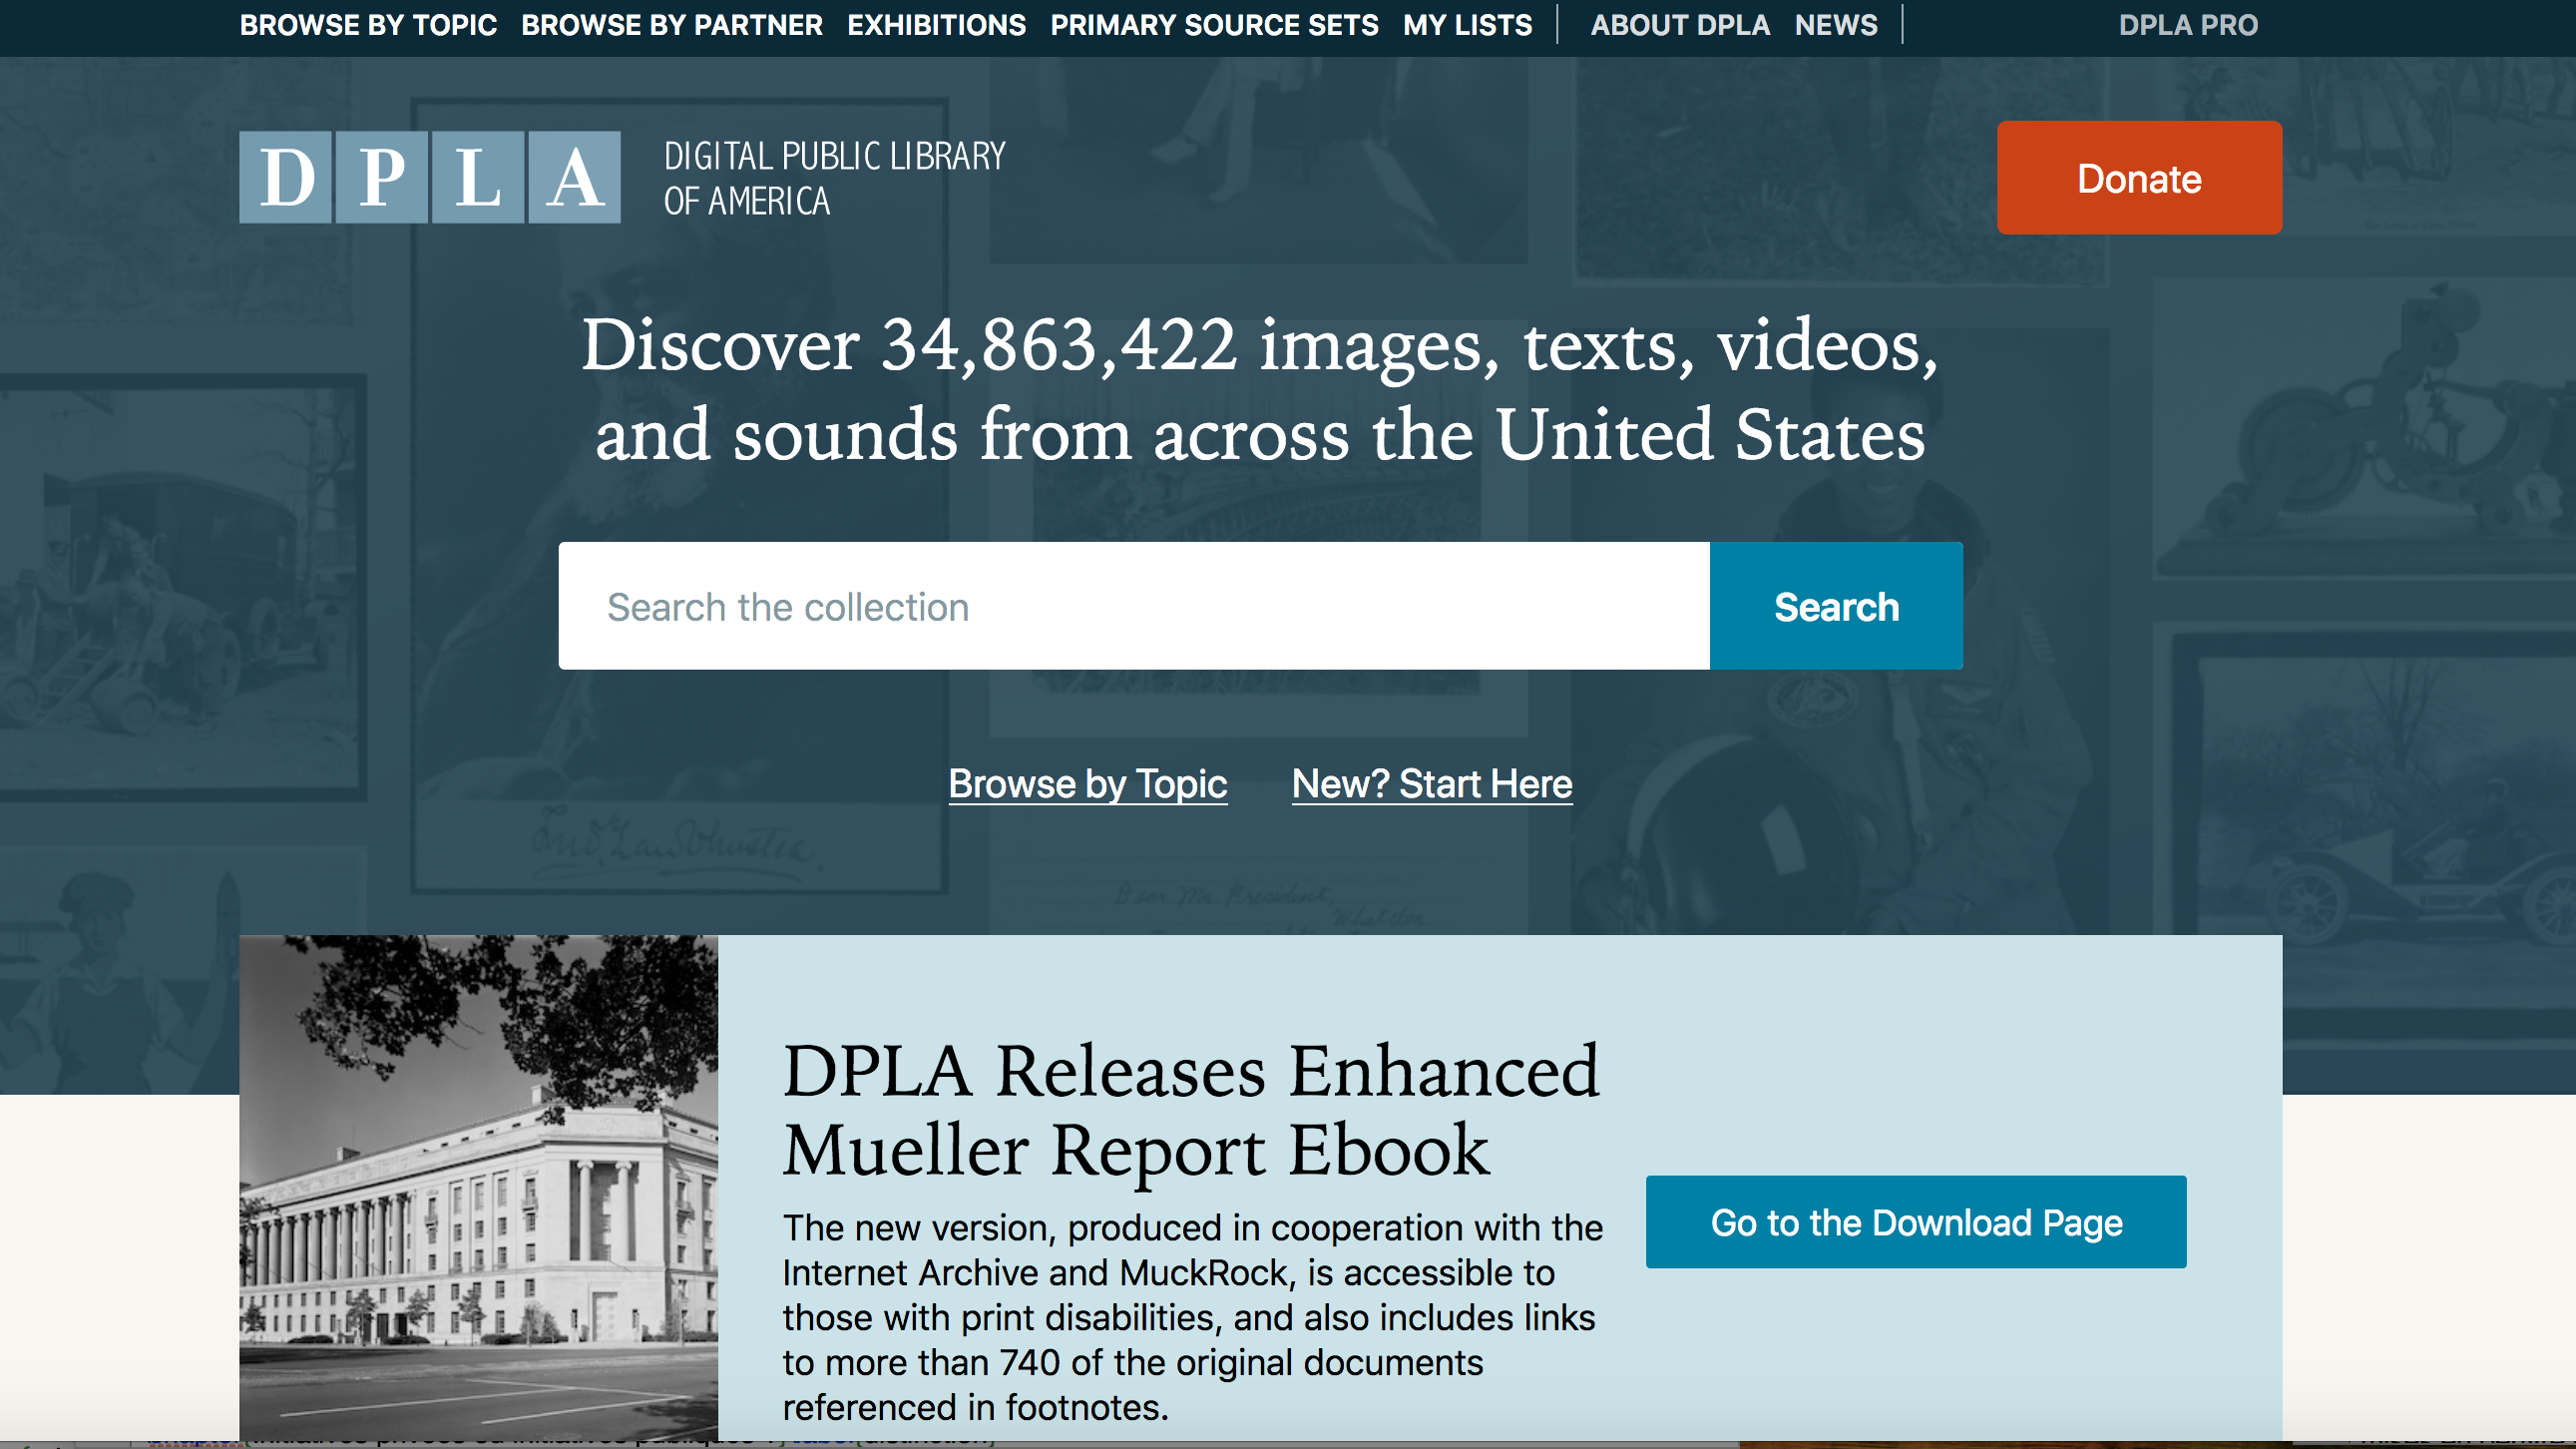
\includegraphics[width=15cm]{dpla}
\caption{Page d'accueil de l'interface découverte du projet de \gls{dpla}, capture d'écran}
\end{figure}

Bien que sa structure soit uniquement basée aux États-Unis, \gls{dpla} a été développé pour être interopérable avec Europeana (le même modèle de métadonnées est utilisé\footcite{digital_public_library_of_america_metadata_nodate}, les deux institutions collaborent au sein du \textit{RightsStatements.org} Consortium etc.). Les liens entre les deux initiatives contribuent ainsi à la création d'un réseau mondial\footcite{xie_discover_2016} et les placent à l'avant-garde d'un mouvement grandissant, visant à proposer des modèles de métadonnées spécifiques à certains domaines\footcite{pomerantz_metadata_2015}. \gls{dpla} s'appuie également sur un réseau d'\gls{agr}s nationaux qui facilitent l'intégration des données de leurs membres, et proposent des solutions de stockage pour les petites institutions qui n'en disposeraient pas\footcite{digital_public_library_of_america_becoming_nodate}\footcite{xie_discover_2016}. Des \gls{api}s permettent des requêtes sur le contenu et les métadonnées, la plateforme propose également un export total de ses \gls{db}\footcite{xie_discover_2016}.

L'initiative soutient une gestion des risques et l'application du \textit{fair use}, offerte par son ancrage géographique, pour justifier la numérisation des \oe{}uvres orphelines ou dont le libre accès suscite des doutes. Il incite toutefois les institutions à entreprendre des recherches sérieuses afin de déterminer si un contenu est libre de droit ou non, et offre un accompagnement dans cette démarche à ses partenaires\footcite{digital_public_library_of_america_understanding_nodate}. 

\gls{dpla} travaille au développement et à la mise en place de solutions techniques afin de soutenir l'engagement des communautés, la recherche et l'éducation. Ses missions actuelles s'articulent autour de différents projets visant à : favoriser l'usage des ebooks par le grand public et les bibliothèques ; accroître l'emploi des collections par le système éducatif ; clarifier l'usage des \oe{}uvres sous droit ; construire des solutions de dépôt numérique ; améliorer la présence de journaux issus de communautés marginalisées ; former les nouveaux partenaires aux technologies de la plateforme et les soutenir dans leurs entreprises de numérisation\footcite{digital_public_library_of_america_projects_nodate}. 

Tout comme Europeana, l'initiative dispose de deux plateformes, l'une permettant la découverte des collections et la deuxième, professionnelle, s'adressant plus précisément : aux agrégateurs partenaires ; aux candidats à la création d'un nouvel agrégateur ; aux communautés de développeurs ; aux chercheurs ; aux utilisateurs d'ebooks ; aux communautés de volontaires souhaitant promouvoir le projet \footcite{digital_public_library_of_america_our_nodate}. Soucieuse de faciliter l'accès à ses collections, la plateforme publique propose également des expositions virtuelles et a développé un \textit{Bot}\footnote{Programme autonome capable d'interagir avec un système ou un utilisateur.} afin de ramener la notion de sérendipité dans la découverte\footcite{thylstrup_politics_2018}.

 \begin{figure}[H]% force à placer l'image au sein de notre balise figure
\centering
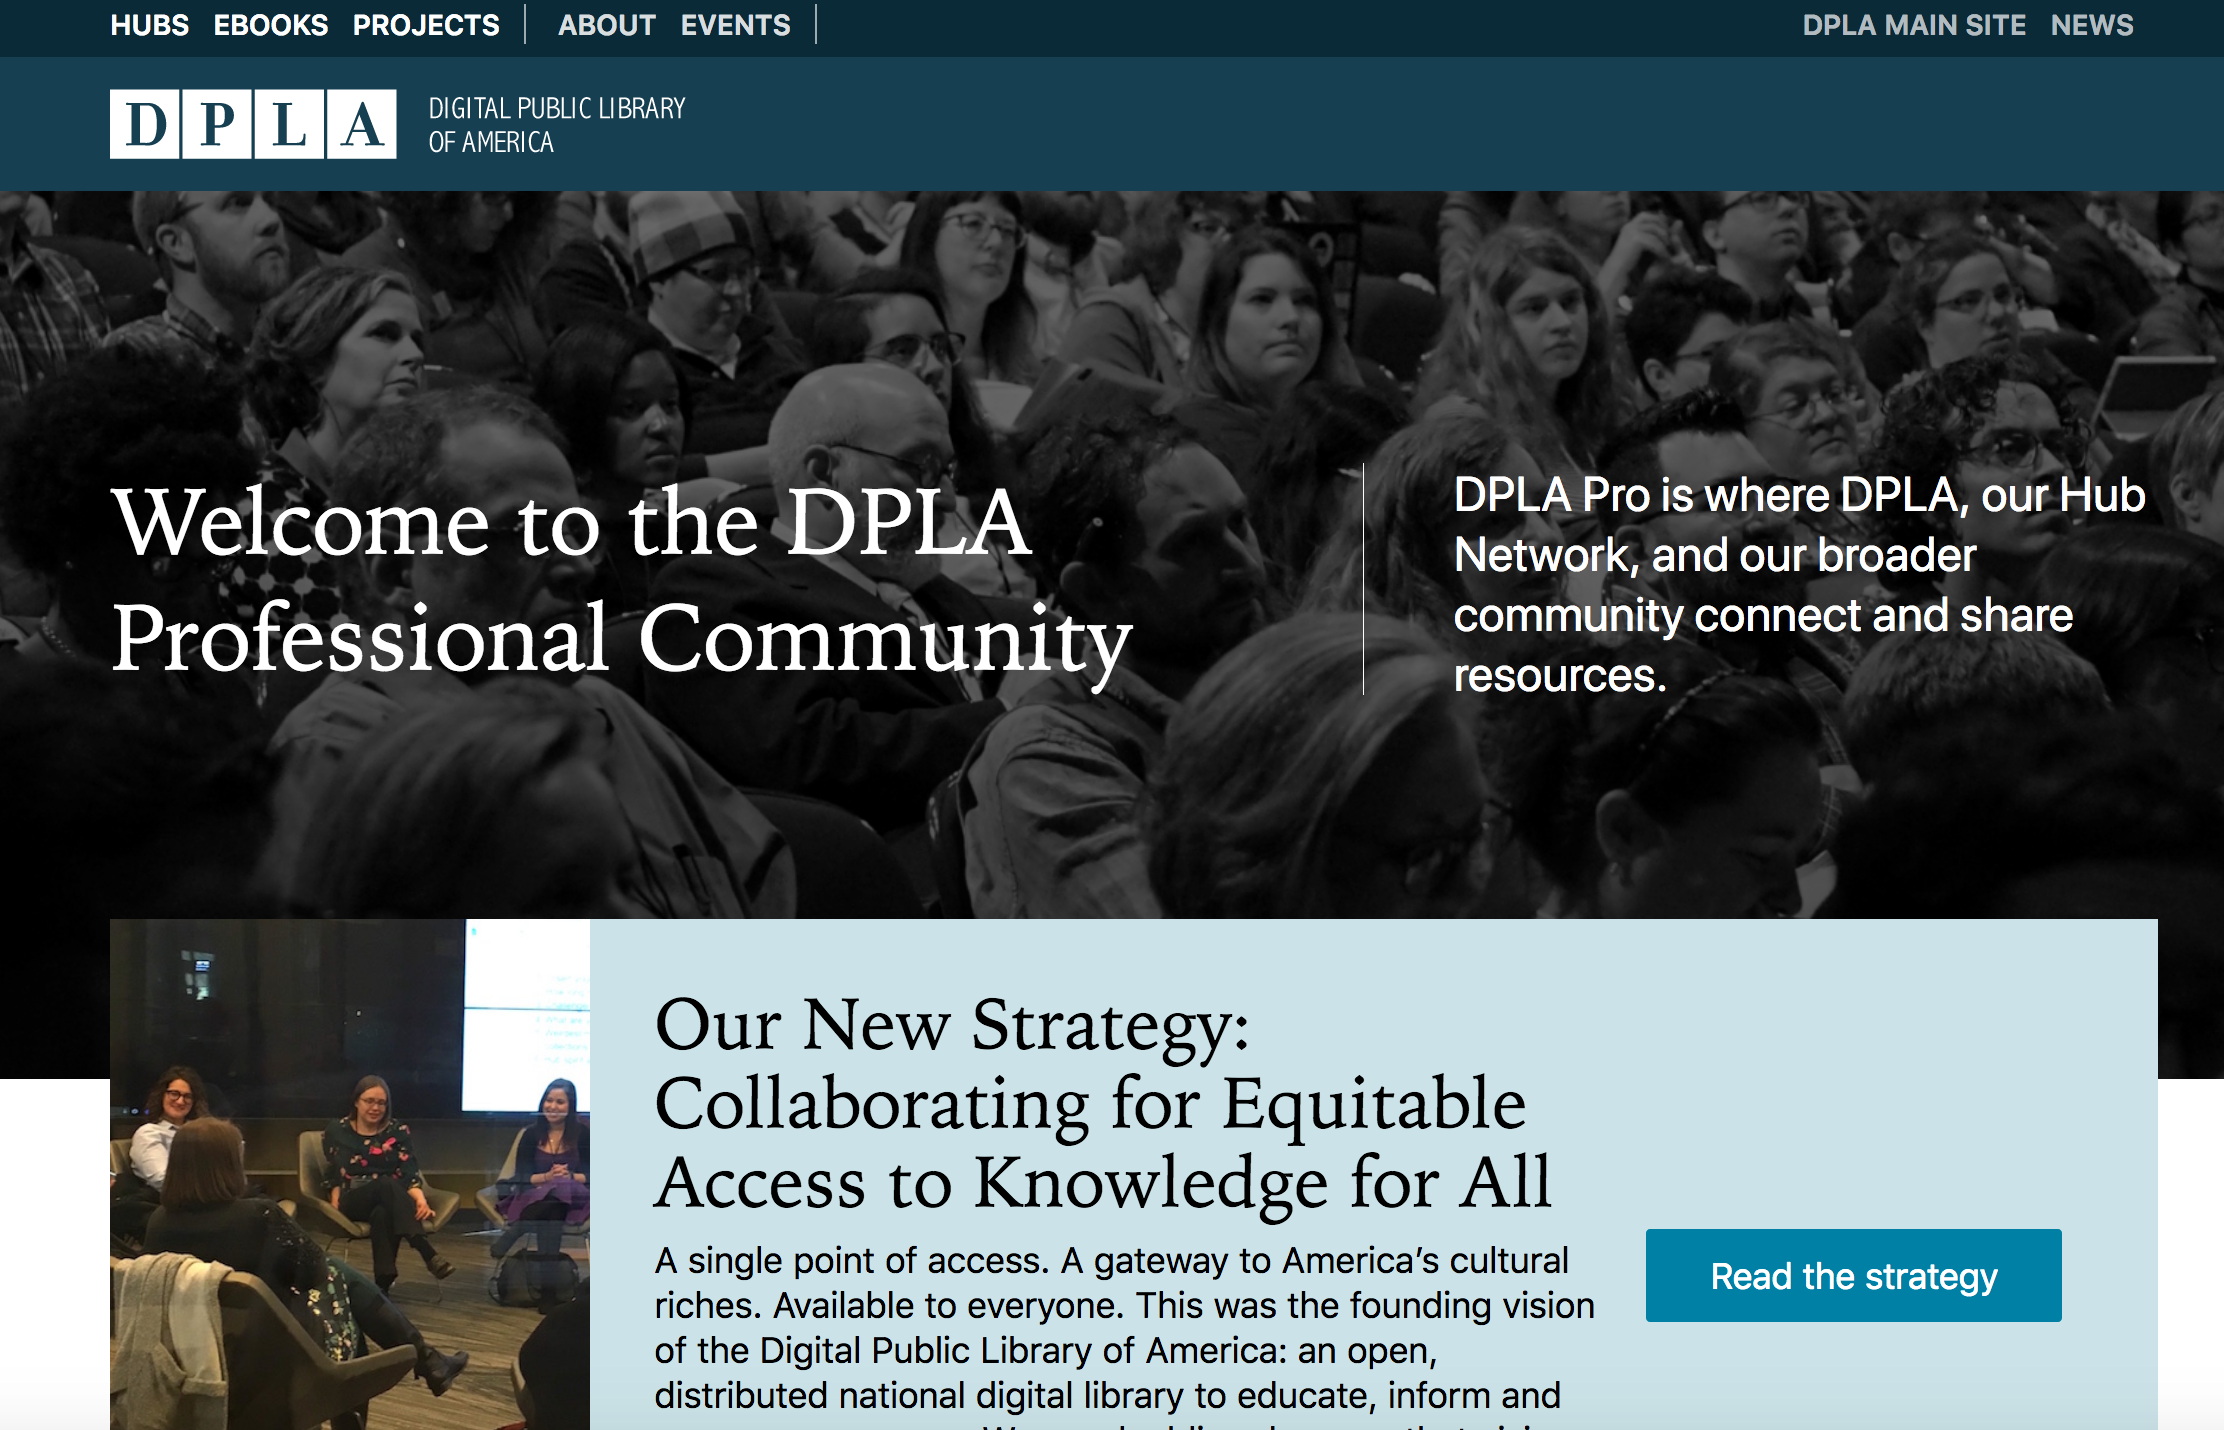
\includegraphics[width=15cm]{dplapro}
\caption{Page d'accueil de l'interface professionnelle du projet de \gls{dpla}, capture d'écran}
\end{figure}

Ces projets et l'infrastructure sont financés par des fondations à but non lucratif, par des fonds du gouvernement américain et par une redevance prélevée auprès des institutions partenaires (qui varie entre 10'000 et 15'000 USD par an)\footcite{digital_public_library_of_america_membership_nodate}. Les institutions doivent elles-mêmes assurer les fonds nécessaires à la numérisation de leurs données mais peuvent être aidées dans cette recherche\footcite{digital_public_library_of_america_our_nodate-1}. Le projet indexe également des données numérisées par Google et stockées par \textit{HathiTrust}.

La collaboration fait partie intégrante de sa démarche, de nombreux groupes de travail sont mis en place afin de réfléchir aux développements de nouvelles solutions. Loin d'être partenaire du clivage Amérique - Europe, l'institution chercher à collaborer avec les réseaux existants\footcite{digital_public_library_of_america_our_nodate}. 
\newpage
\begin{table}[H]
\centering
\begin{tabular}{|l|l|}
\hline
\rowcolor[HTML]{2E1A46} 
{\color[HTML]{FFFFFF} \textbf{Enjeux}}                                                                                   & {\color[HTML]{FFFFFF} \textbf{Réponses de the Digital Public Library of America}}                                                                                                                                                                                                                                                                                                              \\ \hline
{\color[HTML]{2E1A46} \textbf{\begin{tabular}[c]{@{}l@{}}Amener différents\\ acteurs à collaborer\end{tabular}}}         & \begin{tabular}[c]{@{}l@{}}Collaborer fait partie des missions du projet. Une \\ plateforme professionnelle garantit la transparence de la\\ gouvernance. Différents groupes de travail permettent aux \\ partenaires de participer aux développements futurs. Les \\ communautés professionnelles, ou non, sont impliquées dans \\ le projet.\end{tabular}                                    \\ \hline
{\color[HTML]{2E1A46} \textbf{\begin{tabular}[c]{@{}l@{}}Financement et \\ partenariats \\ public-privé\end{tabular}}} & \begin{tabular}[c]{@{}l@{}}Le financement est assuré par le gouvernement américain, \\ des fondations à but non lucratif et une redevance versée\\ annuellement par les partenaires. Les projets de numérisation\\ sont à la charge des partenaires qui peuvent collaborer avec \\ des groupes privés (tels Google, Microsoft etc.).\end{tabular}                                              \\ \hline
{\color[HTML]{2E1A46} \textbf{Droit d'auteur}}                                                                           & \begin{tabular}[c]{@{}l@{}}Favorable à l'usage des licences \textit{Creative Commons}, encourage les \\ partenaires à tirer parti du \textit{fair use} et à mettre en place une gestion \\ des risques. Membre du \textit{RightsStatements}, le projet propose des\\ déclarations de droit standardisées.\end{tabular}                                                                                                  \\ \hline
{\color[HTML]{2E1A46} \textbf{\begin{tabular}[c]{@{}l@{}}Sortir des silos : \\ enjeux techniques\end{tabular}}}          & \begin{tabular}[c]{@{}l@{}}Adoption du modèle de métadonnées développé par \\ Europeana et interopérabilité avec sa plateforme. \\ APIs pour accéder aux métadonnées ou aux contenus.\end{tabular}                                                                                                                                                                                             \\ \hline
{\color[HTML]{2E1A46} \textbf{\begin{tabular}[c]{@{}l@{}}Sortir des silos : \\ enjeux sur le \\ contenu\end{tabular}}}   & \begin{tabular}[c]{@{}l@{}}Hérite des biais des institutions partenaires et sur-représentation de \\ certains formats de documents (textes et images). Un effort est fait \\ pour identifier les manques des collections et les corriger par la mise en \\ place de projets de numérisation ciblés.\end{tabular}                                                                               \\ \hline
{\color[HTML]{2E1A46} \textbf{\begin{tabular}[c]{@{}l@{}}Stockage sur le \\ long-terme - \\ préservation\end{tabular}}}  & \begin{tabular}[c]{@{}l@{}}Développe des solutions de dépôts institutionnels pour les petites\\ institutions et favorise les agrégateurs qui en proposent à leurs \\ communautés. Le stockage des données sur le long-terme demeure\\ sous la responsabilité des institutions. La qualité des métadonnées\\ favorisent le respect de l'intégrité et de l'authenticité des objets.\end{tabular} \\ \hline
\end{tabular}\caption {Les réponses de la \textit{Digital Public Library of America} aux enjeux de la numérisation}
\end{table}
\newpage

% Initiatives publiques versus initiatives privées
\chapter{Comment catégoriser ?}\label{distinction}

La comparaison plus détaillée de ces quatre initiatives de numérisation de masse permet de nuancer les propos de ceux qui distinguent initiatives financées par des institutions commerciales de celles financées par des institutions publiques ou à but non lucratif, puisque les activités de ces deux typologies de projet semblent étroitement imbriquées. Nous appuyons la réflexion contenue dans cette section sur les réponses apportées aux enjeux de la numérisation, bien que d'autres critères non étudiés dans le cadre de ce mémoire auraient pu servir à cette comparaison (tels que le rôle joué par l'homme au sein de ces projets, le nombre de publications officielles proposées etc...)\footcite{leetaru_mass_2008}. 

Les critères proposés par Cory Lampert argumentent que les premières (financées par des institutions commerciales) se distinguent par un enjeu plus grand sur l'accessibilité des données, lorsque les deuxièmes (financées par le secteur public) offrent une modération humaine dans la gestion des collections avec un accent plus développé sur les questions de préservation et la réutilisation des métadonnées\footnote{\cite[p.47]{lampert_ramping_2018}}. Bien que corroborées en un sens par nos exemples, l'analyse de Cory Lampert semble oser quelques raccourcis et ne pas refléter la complexité des réponses apportées aux enjeux de la numérisation. Si \textit{Google Books} offre l'avantage de pouvoir rendre accessible ses données au sein de son propre environnement et bénéficie de fait d'une meilleure visibilité, les autres projets déploient de grands efforts pour améliorer l'accessibilité des leurs. Les différents développements des plateformes d'Europeana, \textit{HathiTrust} et \gls{dpla} témoignent de leurs investissements. Ces trois initiatives se distinguent d'ailleurs par la prise en compte de plusieurs typologies de public et le déploiement de services spécialement adaptés. En ce sens, il est vrai que la modération humaine joue un rôle important pour les initiatives publiques. La préservation n'est certes pas considérée par Google, mais hormis \textit{HathiTrust}, Europeana et \gls{dpla} semblent surtout déléguer cette responsabilité aux institutions détentrices des données. Leur position d'\gls{agr} justifie la réutilisation des métadonnées, afin de ne pas refaire à double le travail mené par leurs institutions partenaires, et constitue plus une conséquence qu'une véritable opportunité.

S'il est vrai que les entreprises publiques que sont Europeana, \gls{dpla} et \textit{HathiTrust} sont davantage transparentes concernant  la gouvernance ou le détail de leurs activités, des développements techniques propres à leurs plateformes et des processus de numérisation, demeurent souvent réalisés par des institutions privées et ne sont dès lors que peu documentés puisqu'ils répondent à des enjeux de protections commerciales évidents : \inquote{\textit{[...]the important infrapolitical question in mass digitization, namely, how, why, and when to manage visibilities[...]}\footcite{thylstrup_politics_2018}}. A ce titre, il est possible d'argumenter que Google offre la même ouverture sur son organisation que les initiatives publiques\footcite{leetaru_mass_2008}. 

La collaboration n'a sans doute pas la même valeur pour \textit{Google Books} que pour les autres projets (puisque dirigé par une seule compagnie qui peut imposer les mêmes règles à ses partenaires\footcite{leetaru_mass_2008}), qui doivent amener un grand nombre d'institutions publiques ou privées à collaborer. Les critères économiques semblent toutefois pousser les initiatives à se développer de manière complémentaire et à collaborer entre réseaux pour trouver des solutions communes (\gls{dpla} et Europeana dans le cadre du \textit{RightsStatements.org}, Europeana et Google pour le partage de certaines fonctionnalités et l'indexation des données numérisées).

Les projets financés uniquement par des fonds publics peinent à construire sereinement leurs activités, Europeana a souvent été contrainte par les instances politiques à revoir ses objectifs et son positionnement\footcite{thylstrup_politics_2018}. Il semble que pour parvenir à un équilibre sur le long-terme, les institutions doivent déployer des partenariats public-privé ou prélever une redevance auprès de leurs partenaires (\textit{HathiTrust}, \gls{dpla}). De plus l'acte de numérisation est finalement souvent financé par des institutions privées, qui imposent dès lors certaines restrictions d'usage\footcite{thelle_persuasive_2011}. 

Concernant le droit d'auteur, Google, de par son emploi du \textit{fair use}, propose un accès moins restrictif à ses collections que les autres exemples étudiés. De plus il a mis en place avant les autres initiatives différents affichages en fonction des droits liés au document\footcite{leetaru_mass_2008}. \gls{dpla} défend d'ailleurs la mise en place d'une gestion des risques dans les projets de numérisation américains afin de favoriser un accès plus large aux collections potentiellement sous droit. Les différents projets peinent toutefois à proposer une solution satisfaisante, ce qui résulte en une sous-représentation des \oe{}uvres à partir du 20\up{e} siècle. 

La quête de l'interopérabilité est au centre des préoccupations des projets. Si l'environnement de Google permet à \textit{Google Books} de s'affranchir des barrières, \gls{dpla}, Europeana et \textit{HathiTrust} sont contraints de développer plusieurs solutions techniques pour sortir des silos des institutions.

Bien qu'il y ait au sein de toutes les initiatives une volonté officialisée de donner accès à la connaissance qu'elle soit universelle ou européenne, sa définition ne semble pas faire l'unanimité. Google se limite aux livres et restreint sa politique de numérisation à ce format, tandis qu'Europeana et \gls{dpla} en élargissent le champ pour inclure d'autres formes de création. Les critères de sélection liés au développement des collections, mis en place par les institutions, sont reproduits au sein des projets de numérisation de masse, et si certains argumentent que \textit{Google Books} n'a pas de politique documentaire\footcite{dufrene_numerisation_2013}, il en a en vérité une très complexe, au vu du nombre de ses partenaires\footcite{coutts_stepping_2017}. Il est cependant indéniable que certains projets travaillent plus activement à détecter et corriger leurs \inquote{manques}, à l'instar de \gls{dpla} et Europeana. 

\textit{HathiTrust} est le projet le plus actif dans la préservation des données sur le long-terme, puisqu'il s'est construit autour de cette mission et pour pallier au désintérêt montré par Google sur la question. Toutefois les deux initiatives sont les seules à stocker elles-mêmes leurs données numérisées. Europeana et \gls{dpla}, en temps qu'\gls{agr}s semblent surtout déléguer cette responsabilité aux institutions, bien que \gls{dpla} travaille au développement et à l'implémentation de dépôts pour celles qui n'en auraient pas.

Vouloir effectuer une catégorisation entre ces différentes initiatives, semble relever aujourd'hui d'un exercice difficile. La distinction public-privé s'efface au profit d'une collaboration. La proposition de Margaret Coutts que nous avons choisie d'appliquer, bien que cohérente, semble manquer de plus en plus d'initiatives actives au sein du premier groupe et encourt d'une part, le risque d'isoler la démarche d'\textit{HathiTrust} et de restreindre ses activités de valorisation derrière la bannière de la préservation, et d'autre part, d'occulter le rôle joué par Google au sein du deuxième groupe. Les initiatives de numérisation de masse évoluent rapidement et leur croissance continue rend l'exercice de définition de ces géants de plus en plus complexe, tant ils s'articulent autour d'enjeux et d'objectifs multiples\footcite{thylstrup_politics_2018}. 

Peut-être qu'alors il serait plus raisonnable de considérer les projets de numérisation de masse comme un tout, chaque nouvelle initiative se construisant sur les précédentes et contribuant à renforcer les bonnes pratiques et à proposer de nouvelles orientations, plutôt que de vouloir séparer des projets pourtant motivés par les développements des autres. Une approche inclusive de ces initiatives permettrait l'ouverture de nouvelles perspectives de recherches, palliant au risque d'une catégorisation trop réductive incapable de refléter leur envergure.






 










